\section{Overview of single-cell Variational Inference (scVI)}
\subsection{Model definition}

The primary output of an scRNA-seq experiment is an $N \times G$-matrix $x$ that records the number of transcripts measured for each of $G$ genes in each of $N$ cells. We may also have a batch annotation $s_n$ observed for each cell $n$ as well.

We model the  expression level $x_{ng}$ measured for each cell $n$ and gene $g$ as a sample drawn from a conditional distribution that has a zero-inflated negative binomial (ZINB) form \cite{Grun2014,deseq2,zinbwave}. The distribution is conditioned on the observed batch annotation, as well as  two additional, unobserved random variables. The latent random variable $\ell_n$ represents nuisance variation due to variation in capture efficiency and sequencing depth. It is drawn from a log-normal distribution and serves as a cell-specific scaling factor. %Notably, the heavy tail property of $\ell_n$ makes the distribution of gene expression richer and better removes the variation in gene expression coming from library size. %%Not sure about this one. This might open up for a reviewer's question

The latent random variable $z_n$ represents the remaining variability, which should better reflect biological differences between cells. It is drawn from a standard multivariate normal of low dimensionality $d$, and provides a latent-space representation that can be used for visualization and clustering.
The matrix $\rho$ is an intermediate value that relates the observations $x_{ng}$ to the latent variables. It provides a batch-corrected, normalized estimate of the percentage of transcripts in each cell $n$ that originate from each gene $g$. We use $\rho$ for differential expression analysis and its scaled version (multiplying by the estimated library size) for imputation.

Altogether, each expression value $x_{ng}$ is drawn independently through the following process:
\begin{align}
	z_n &\sim \textrm{Normal}(0, I) \\
    \ell_n &\sim \textrm{LogNormal}(\ell_\mu, \ell_\sigma^2) \\
    \rho_n &= f_w(z_n, s_n) \\
    w_{ng} &\sim \mathrm{Gamma}(\rho_n^g, \theta) \\
    y_{ng} &\sim \mathrm{Poisson}( \ell_n w_{ng}) \\
    h_{ng} &\sim \mathrm{Bernoulli}(f_h^g(z_n, s_n)) \\
    x_{ng} &=
\begin{cases}
y_{ng} & \text{ if } h_{ng} = 0,\\
0 & \text{ otherwise}.\\
\end{cases}
\end{align}
A standard multivariate normal prior for $z$ is commonly used in variational autoencoders since it can be reparametrized in a differentiable way into any arbitrary multivariate Gaussian random variable~\cite{kingma2013}, which turns out to be extremely convenient in the inference process. 

$B$ denotes the number of batches and $\ell_\mu, \ell_\sigma \in \mathbb{R}_+^B$ parameterize the prior for the scaling factor (on a log scale), and are set to be the empirical mean and variance of the log-library size per each batch. Let us note that the random variable $\ell_n$ is not the log-library size (scaling the sampled observation) itself but a scaling factor that is expected to correlate strongly with log-library size (hence the choice of the parameters).

The parameter $\theta \in \mathbb{R}_+^G$ denotes a gene-specific inverse dispersion, are estimated as global parameters estimated via variational Bayesian inference. $f_w$ and $f_h$ are neural networks that map the latent space and batch annotation back to the full dimension of all genes: $\mathbb{R}^d\times\{0, 1\}^B \rightarrow \mathbb{R}^G$ (Figure 1b, NN5-6). We use superscript annotation (e.g., $f_w^g(z_n, s_n)$) to refer to a single entry that corresponds to a specific gene $g$. We apply a softmax activation at the last layer of $f_w$. Therefore, $f_w^g(z_n, s_n)$ to take values in the probability simplex (namely, for each cell $n$ the sum of $f_w^g(z_n, s_n)$ values over all genes $g$ is one), and may be interpretated as expected frequencies. Neural network $f_h$ encodes whether a particular entry has been dropped out due to technical effects~\cite{zifa,zinbwave}. Importantly, neural networks allows us to go beyond the generalized linear model framework and provide a more flexible model of gene expression. Figure \ref{scviPanel1}a specifies the complete graphical model and its implementation using neural-network conditionals.

All neural networks use dropout regularization and batch normalization. Each network has 1, 2, or 3 fully connected-layers, with 128 or 256 nodes each. The activation functions between two hidden layers are all ReLU. We use a standard link function to parametrize the distribution parameters (exponential, logarithmic or softmax). Weights for some layers are shared between $f_w$ and $f_h$. 

\begin{figure}
    \centering
    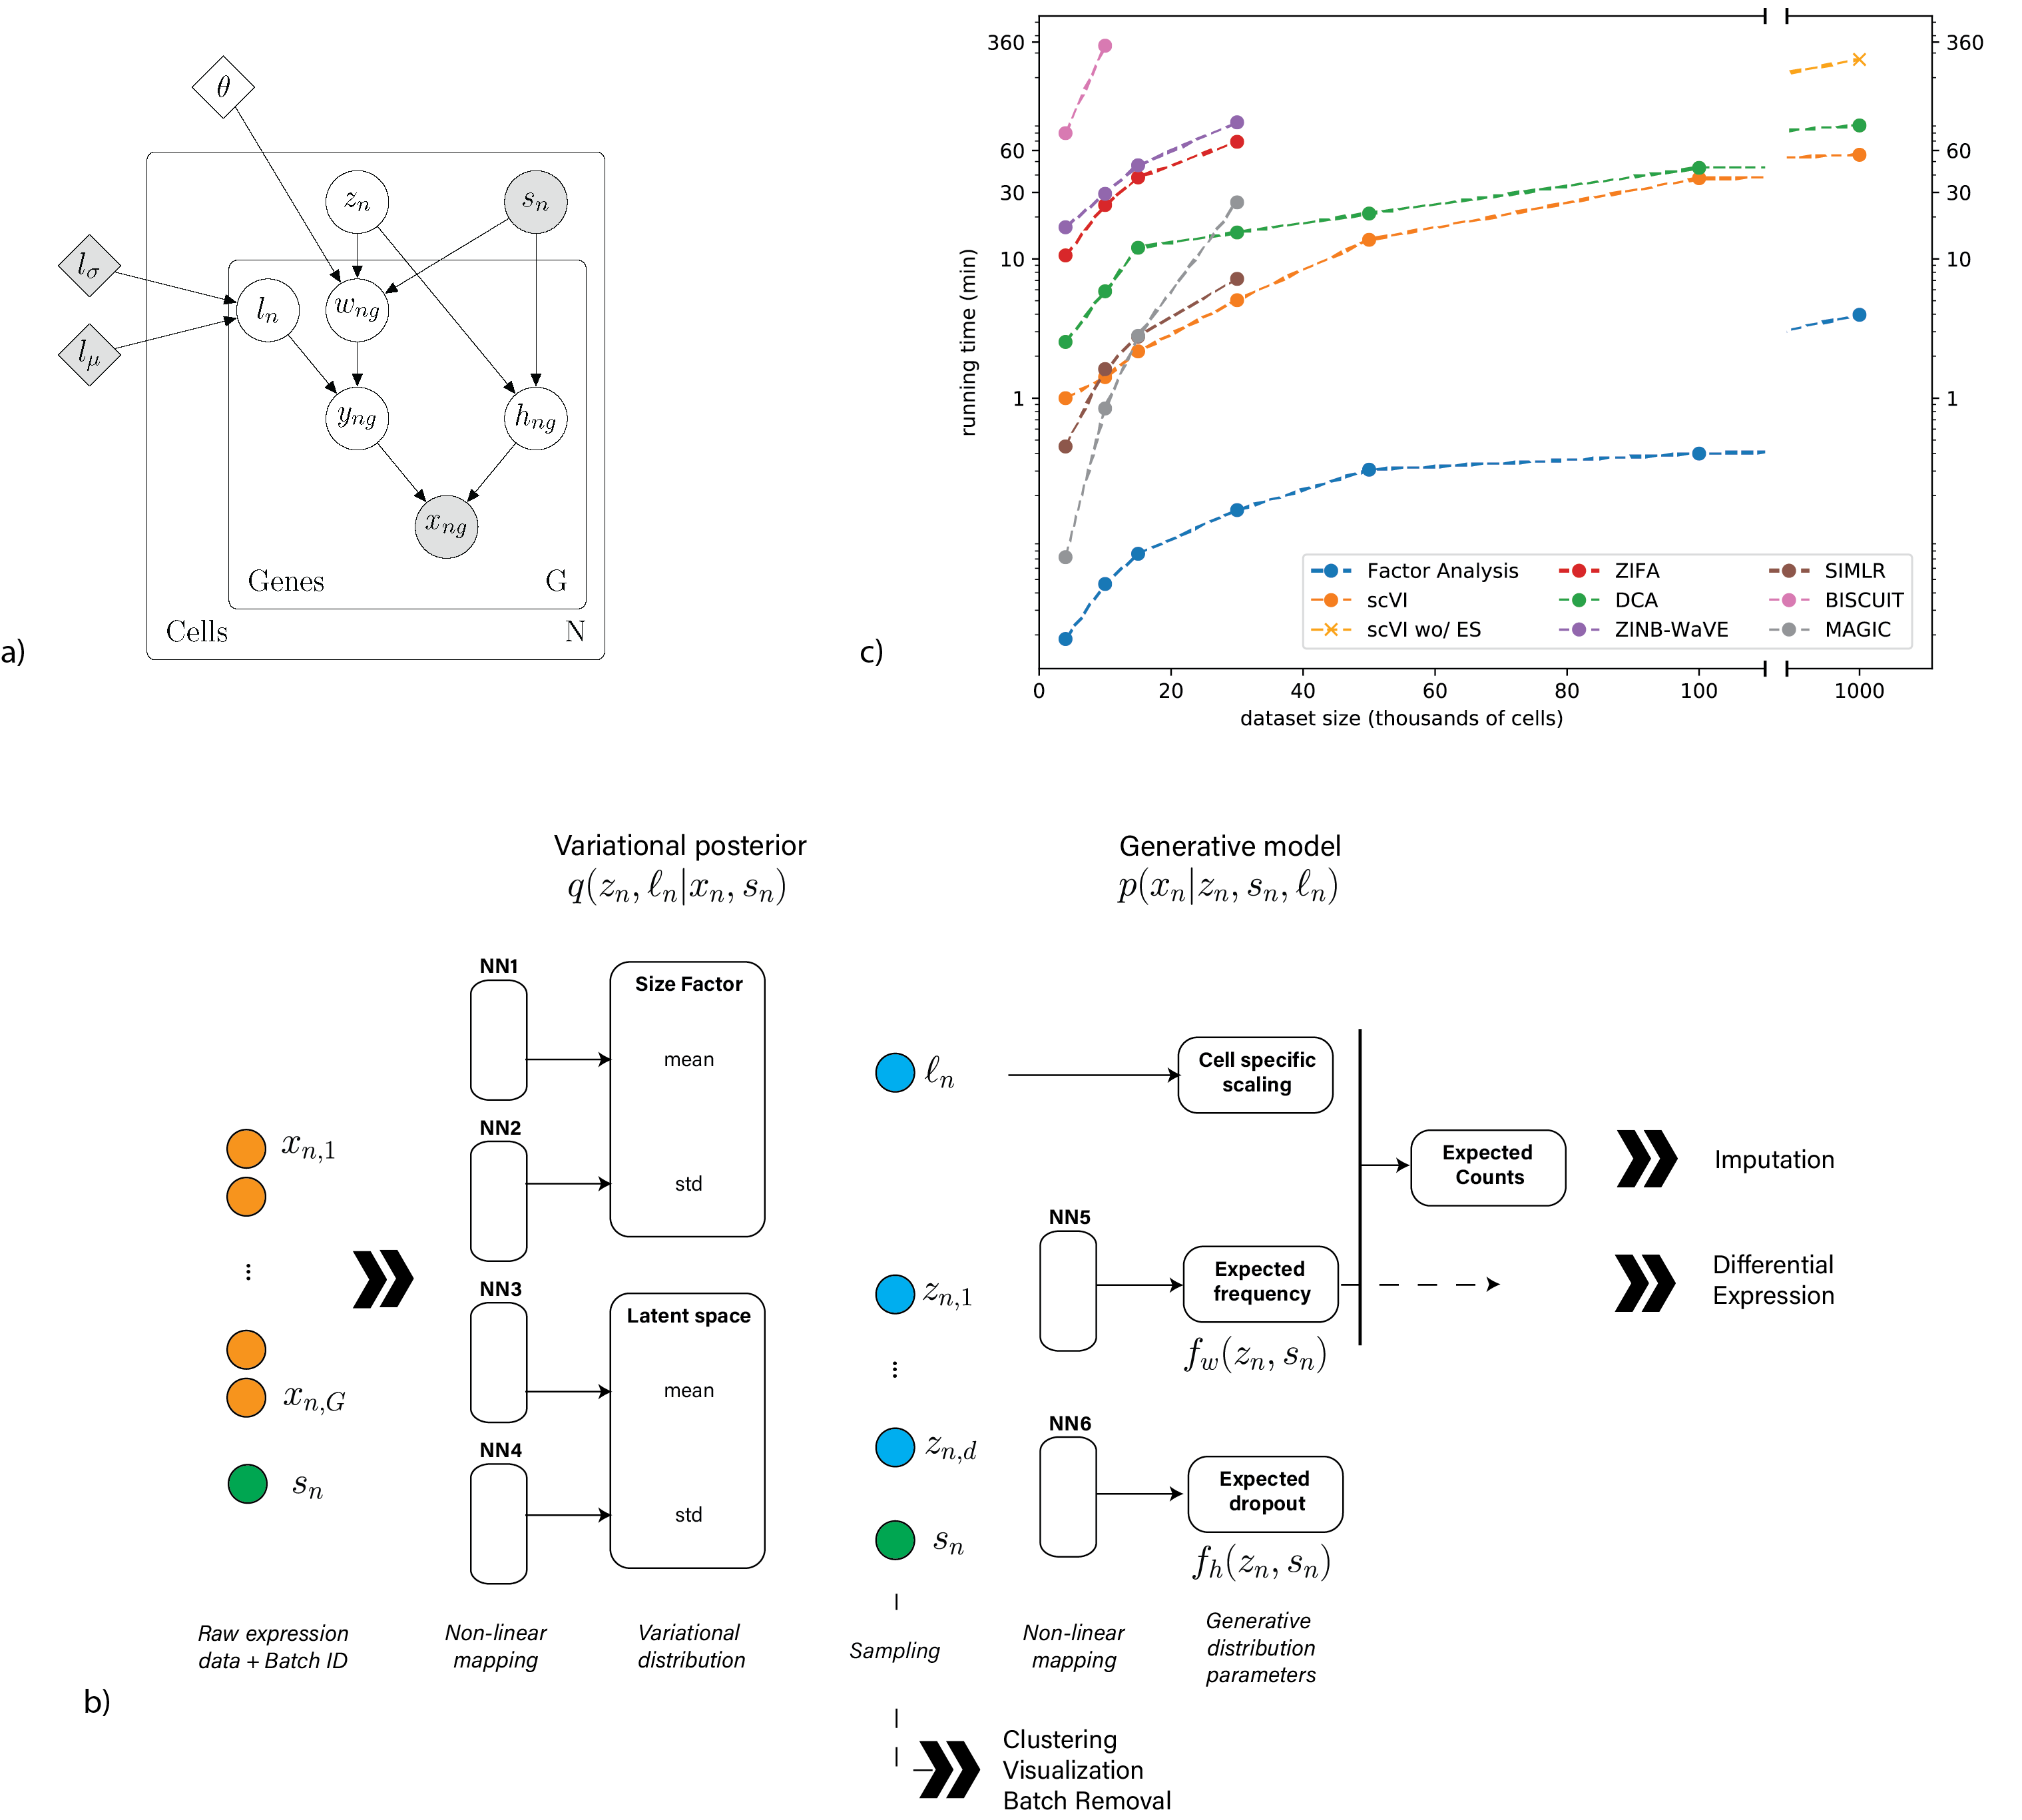
\includegraphics[width=0.9\textwidth]{figures/Figure-1.png}
    \caption[Overview of scVI]{Overview of scVI. Given a gene-expression matrix with batch annotations as input, scVI learns a non-linear embedding of the cells that can be used for multiple analysis tasks. (a) The underlying graphical model. Shaded vertices represent observed random variables. Empty vertices represent latent random variables. Shaded diamonds represent constants, set a priori. Empty diamonds represent global variables shared across all genes and cells. Edges signify conditional dependency. Rectangles (``plates'') represent independent replication. (b) The computational trees (neural networks) used to compute the embedding as well as the distribution of gene expression. (c) Comparison of running times (y-axis) on the BRAIN-LARGE data with a limited set of 720 genes, and with increasing input sizes (x-axis; cells in each input set are sampled randomly from the complete dataset). scVI is compared against existing methods for dimensionality reduction in the scRNA-seq literature. As a control, we also add basic matrix factorization with factor analysis (FA). For the one-million-cell dataset only, we report the result with and without early stopping (ES).}
    \label{scviPanel1}
    \end{figure}
    

\subsection{Fast inference via stochastic optimization}
The posterior distribution combines the prior knowledge with information acquired from the data $X$. We cannot directly apply Bayes rule to determine the posterior because the denominator (the marginal distribution) $p(x_n \mid s_n)$ is intractable. We therefore proceed to deriving a variational inference recipe. 

\subsubsection{Partial analytical integration of latent variables}
Making inference over the whole graphical model is not needed. We can integrate out the latent variables $w_{ng}$, $h_{ng}$ and $y_{ng}$ by ensuring the conditional $p(x_{ng} \mid z_{n}, \ell_{n}, s_n)$ has a closed-form density and is zero-inflated negative binomial. The result follows from analytical integration:

\begin{restatable}{lemma}{lemmazinb}\emph{(Marginalizing the latent variables of scVI)}\label{lemma:zinb}
    The conditional distribution $p(x_{ng} \mid z_{n}, \ell_{n}, s_n)$ follows a zero-inflated negative binomial distribution of mean $\ell_{n}f^g_w(z_n, s_n)$, dispersion $\theta_g$ and mixture weight $f^g_h(z_n, s_n)$.
    \end{restatable}
\begin{proof}
    For this proof, we need to first apply a standard result on Gamma poisson compounds, and then carefully identify the zero probability. 
    \paragraph{Step 1: integrating the Gamma latent variable} Let $r$ to be the gene-specific shape parameter of a Gamma variable $w$ and let $\frac{p}{1-p}$ be its scale parameter. For any scalar $\lambda \in \mathbb{R}^+$, the random variable defined by $y \mid w \sim \textrm{Poisson}(\lambda w)$ has a negative binomial marginal distribution with mean $\lambda\frac{rp}{1-p}$ and shape $r$:
\begin{align}
 p(y) &= \int p(y \mid w) p(w)dw  \\
 &= \int \frac{w^{r-1} e^{-w(\frac{1}{p}-1)}(1-p)^r}{p^r\Gamma(r)}\frac{e^{-\lambda w} \lambda^y w^y}{\Gamma(y+1)}dw \\
&= \frac{\Gamma(y + r)}{\Gamma(y+1)\Gamma(r)} \left(\frac{1-p}{1-p + \lambda p} \right)^r \left(\frac{p\lambda}{1-p + \lambda p} \right)^y \\
&= \textrm{NegativeBinomial}\left(y; \lambda\frac{rp}{1-p}, r\right).
\end{align}
\paragraph{Step 2: identifying the zero-probability}
Multiplication by zero to $y_{ng}$ can be formally encoded as a mixture between a point-mass at zero and the original distribution of $y_{ng}$. Then, our conditional $p(x_{ng} \mid z_{n}, \ell_{n}, s_n)$ is a zero-inflated negative binomial:
\begin{align}
       p(x_j = 0 \mid z, l, s) &= f_h(z)_j + (1 - f_h(z)_j) \left( \frac{\theta_j}{\theta_j + l f_w(z)_j } \right)^{\theta_j}
\end{align}
and
\begin{align}
      p(x_j = y \mid z, l, s) &= (1-f_h(z)_j) \frac{\Gamma(y + \theta_j)}{\Gamma(y+1)\Gamma(\theta_j)} \left( \frac{\theta_j}{\theta_j + l f_w(z)_j } \right)^{\theta_j} \left( \frac{lf_w(z)_j}{\theta_j + l f_w(z)_j } \right)^y.
\end{align}
Here $f_h(z)$ encodes the zero probability of $h$ and $f_w(z)$ the mean of $w$.
\end{proof}

\subsubsection{Amortized variational inference}
Having simplified our model, we use variational inference~\cite{blei2017variational} to approximate
the posterior $p(z_n, \ell_n \mid x_n, s_n)$. Our variational distribution $q(z_n, \ell_n \mid x_n, s_n)$ is mean-field:
\begin{align}
    q(z_n, \ell_n \mid x_n, s_n) = q(z_n \mid x_n, s_n)q(\ell_n \mid x_n, s_n).
\end{align}

The variational distribution $q(z_n \mid x_n, s_n)$ is chosen to be Gaussian with a diagonal covariance matrix, mean
and covariance given by an encoder network applied to $(x_n, s_n)$, as in~\cite{kingma2013} (Figure 1b, NN1-4)). The variational distribution $q(\ell_n \mid x_n, s_n)$ is chosen to be log-normal with the scalar mean and variance also given by an encoder network applied to $(x_n, s_n)$. The variational lower bound is:
\begin{equation}\label{scvivar_bound}
\begin{split}
\log p(x_n \mid s_n) \geq & \mathbb{E}_{q(z_n, l_n\mid x_n, s_n)}\log p(x_n\mid z_n, l_n, s_n)  \\
& \qquad- \kld{q(z_n\mid x_n, s_n)}{p(z_n)} \\
& \qquad - \kld{q(l_n\mid x_n, s_n)}{p(l_n)}.
\end{split}
\end{equation}

In this objective function, the dispersion parameters $\theta_g$ for each gene  are treated as global variables to optimize in a Variational Bayesian inference fashion. To optimize the lower bound, we use the analytic expression for $p(x_n\mid z_n, l_n, s_n)$ and use analytic expressions for the Kullback-Leibler divergences. We use the reparametrization trick to compute low-variance Monte-Carlo estimates of the expectations' gradients. Analytic closed-form for the Kullback-Leibler divergence and the reparametrization trick are only possible on certain distributions which multivariate Gaussians are a part of~\cite{kingma2013}. Now, our objective function is continuous and end-to-end differentiable, which allows us to use automatic differentiation operators. As indicated in \cite{Sønderby2016}, we use deterministic warmup and batch normalization during learning to learn an expressive model.

Since our model assumes cells are identically independently distributed, we can also benefit from stochastic optimization by sampling the training set. We then have an online optimization procedure that can handle massive datasets. At each iteration, we focus only on a small subset of the data randomly sampled ($M = 128$ data points) and do not need to go through the entire dataset. Therefore, there is no need to store the entire dataset in memory. Because the number of genes is  in practice limited to a few tens of thousands, these mini-batches of cells fit easily into a GPU.

Since the encoder network $q(z \mid x, s)$ might still produce output correlated with the bath $s$, we use a Maximum Mean Discrepancy (MMD) based penalty as in \cite{louizos2016variational} to correct the variational distribution. For this chapter, however, we did not explicitly enforce the MMD penalty and simply retained the conditional independence property, which has shown to be sufficiently efficient. This may be useful on other datasets.

\subsection{Choice of hyperparameters}
Throughout the chapter, we use Adam (a first order stochastic optimizer) with $\epsilon = 0.01$. A complete list of datasets and their properties, the methods we applied, and a complete list of hyperparameters is provided in Table \ref{scvidatasets}. The hyperparameters were chosen using a small grid search that maximized held-out log likelihood---a common practice for training deep generative models. One of the strengths of scVI is that we have only three dataset-specific hyperparameters to set (learning rate, number of layers, and layer width). We optimize the objective function until convergence  --usually between 120 and 250 epochs, where each epoch is a complete pass through the dataset (let us note that bigger datasets require fewer epochs). For the larger subset of the BRAIN-LARGE dataset, we also ran with the early stopping criterion: the algorithm stops after 12 consecutive epochs with no improvement on the loss. 


\begin{table}
    \centering
    \resizebox{\textwidth}{!}{
        \begin{small}
    \begin{tabular}{lcccccccccc}
    \toprule

                                                                   & \multicolumn{2}{c}{\textbf{dataset properties}} & \multicolumn{3}{c}{\textbf{scVI hyperparameters}}                                                     & \multicolumn{5}{c}{\textbf{scalability to other algorithms}}                                                                 \\
    \textbf{}                                                      & \textbf{cells}         & \textbf{genes}         & \textbf{\begin{tabular}[c]{@{}l@{}}learning\\ rate\end{tabular}} & \textbf{layers} & \textbf{neurons} & \textbf{FA} & \textbf{ZIFA} & \textbf{\begin{tabular}[c]{@{}l@{}}ZINB\\ WaVE\end{tabular}} & \textbf{MAGIC} & \textbf{SIMLR} \\
    \midrule \\
    \textbf{CORTEX}                                                & 3,005                  & 558                    & 0.0004                                                           & 1               & 128              & \_          & \_            & \_                                                           & \_             & \_             \\[0.2cm]
    \textbf{PBMC}                                                  & 12,039                 & 3,346                  & 0.0004                                                           & 1               & 128              & \_          & x             & x                                                            & \_             & \_             \\[0.2cm]
    \textbf{HEMATO}                                                & 4,016                  & 7,397                  & 0.0004                                                           & 1               & 128              & \_          & x             & x                                                            & \_             & NC             \\[0.2cm]
    \textbf{HEMATO$^*$}                                                & 4,016                  & 700                  & 0.0004                                                           & 1               & 128              & \_          & x             & x                                                            & \_             & NC             \\[0.2cm]
    \textbf{\begin{tabular}[c]{@{}l@{}}BRAIN\\ LARGE\end{tabular}} & 10,000                 & 720                    & 0.001                                                            & 1               & 128              & \_          & \_            & \_                                                           & \_             & NA             \\[0.4cm]
    \textbf{\begin{tabular}[c]{@{}l@{}}BRAIN\\ LARGE\end{tabular}} & 15,000                 & 720                    & 0.001                                                            & 2               & 128              & \_          & \_            & \_                                                           & NC             & NA             \\[0.4cm]
    \textbf{\begin{tabular}[c]{@{}l@{}}BRAIN\\ LARGE\end{tabular}} & 50,000                 & 720                    & 0.001                                                            & 3               & 256              & \_          & x             & x                                                            & NC             & NA             \\[0.4cm]
    \textbf{\begin{tabular}[c]{@{}l@{}}BRAIN\\ LARGE\end{tabular}} & 1M                     & 720                    & 0.001                                                            & 3               & 256              & \_          & x             & x                                                            & x             & NA             \\[0.4cm]
    \textbf{\begin{tabular}[c]{@{}l@{}}BRAIN\\ LARGE\end{tabular}} & 1M                     & 10,000                    & 0.001                                                            & 3               & 256              & \_          & x             & x                                                            & x             & NA             \\[0.4cm]
    \textbf{RETINA}                                                & 27,499                 & 13,166                 & 0.0005                                                           & 1               & 128              & \_          & x             & x                                                            & x              & \_             \\[0.2cm]
    \textbf{CBMC}                                                  & 8,617                  & 600                    & 0.0005                                                           & 1               & 128              & \_          & \_            & \_                                                           & NC             & \_             \\[0.2cm]
    \textbf{\begin{tabular}[c]{@{}l@{}}BRAIN\\ SMALL\end{tabular}} & 9,128                  & 3,000                  & 0.001                                                            & 1               & 128              & NC          & NC            & NC                                                           & NC             & NC\\
    \bottomrule
\end{tabular}
\end{small}
    }
    \caption[Presentation of the different datasets, their gene filtering and applicability of algorithms]{Presentation of the different datasets, their gene filtering and applicability of algorithms. ``\_'' indicates combinations of algorithms and datasets that were included in this study. ``x'' indicates that the algorithm took more than four hours to run (ZIFA) or that the computer ran out of memory (others). ``NA'' indicates datasets where pre-annotated subpopulations were not available, which makes them less useful for application with SIMLR and benchmarks of clustering. ``NC'' indicates the remaining combinations of algorithms and datasets that were not considered for this study. For instance, BRAIN-SMALL was only used to study the correlation of scVI zero probabilities and quality parameters (Figure 6).}
    \label{scvidatasets}
    \end{table}
    

    


\subsection{Related variational autoencoder works}
Independently of our work, several recent articles and preprints have also described the use of neural networks, including variational autoencoders~\cite{kingma2013} (VAEs), to embed scRNA-seq datasets. Like scVI, these methods use stochastic optimization and therefore also scale to the size of recent data sets. 
scVI stands apart from this research in its focus on separating technical effects from biological signals. To this end, we explicitly model library size and batch effects as nuisance variables in a hierarchical Bayesian model. Empirical advantages of such careful modeling are underlined in~\cite{biscuit,basics} for library size and~\cite{zinbwave,SCONE} for batch effects. scVI is also distinguished by the large variety of datasets it has been validated on, and the number downstream applications it supports (see Table~\ref{scvialgorithms_pres}). In the following, we provide a brief description of each method.

scvis~\cite{scvis} proposes a new variational lower bound inspired by the parametric version of tSNE for single-cell visualization. Unlike scVI, scvis uses principal component analysis for preprocessing the data, and relies on $t$-distributed conditional distributions. These assumptions may be fruitful for visualization purposes but may not help in recovering hidden gene expression levels for either imputation or differential expression. One notable reason is that the underlying statistical assumptions for applying principal component analysis are not verified in the scRNA-seq dataset and the output of this preprocessing may have artifacts~\cite{zinbwave}.

VASC~\cite{VASC} adds zero-inflation to a VAE with Gaussian conditional distributions and shows competitive performance on clustering. Preprocessing relies on normalizing the data by library size in order to suit their loss function. However, it is known that size scaling normalization can induce bias in the analysis~\cite{vallejos2017normalizing} and that count distributions such as ZINB outperform zero-inflated Gaussian conditional distribution for modeling and downstream analysis~\cite{zinbwave, zifa}.

DCA~\cite{dca} is a denoising auto-encoder~\cite{VincentPASCALVINCENT2010} that proposes a ZINB loss function. The output of this algorithm is a latent space as well as a point estimate for the conditional distributions (this denoising method is essentially a non-linear version of ZINB-WaVE). However, it is hard to extend this method for differential expression without the possibility of posterior sampling. Notably, library size discrepancies are also corrected via size scaling and potentially hurt downstream analysis~\cite{vallejos2017normalizing}.

scVAE~\cite{scVAE} proposes to use VAEs with count conditional distributions for Bayesian modeling and clustering analysis. Notably, their work uses (among others) the NB and the ZINB as conditional distributions but do not propose an approach for normalization, which is crucial for further analysis.

\begin{table}
\centering
\resizebox{\textwidth}{!}{
    \begin{small}
\begin{tabular}{lcccccccc}
    \toprule
                         & \multicolumn{5}{c}{\textbf{Characteristics of the Model}}                                                                                                                                                                                                  & \multicolumn{3}{c}{\textbf{Features of the Software}}                                                                                                                            \\
                        \\
                         & \textbf{Dropout} & \textbf{\begin{tabular}[c]{@{}l@{}}Count\\ distribution\end{tabular}} & \textbf{Library size} & \textbf{\begin{tabular}[c]{@{}l@{}}Batch \\ Effects\end{tabular}} & \textbf{\begin{tabular}[c]{@{}l@{}}Generative\\ Model\end{tabular}} & \textbf{\begin{tabular}[c]{@{}l@{}}Dimensionality \\ Reduction\end{tabular}} & \textbf{Imputation} & \textbf{\begin{tabular}[c]{@{}l@{}}Differential\\ Expression\end{tabular}} \\
   \midrule                      
\textbf{Factor Analysis} &                  &                                                                       &                       &                                                                   & X                                                                   & X                                                                            &                     &                                                                            \\[0.2cm]
\textbf{ZIFA}            & X                &                                                                       &                       &                                                                   & X                                                                   & X                                                                            &                     &                                                                            \\[0.2cm]
\textbf{SIMLR}           &   X               &                                                                       &                       &                                                                   &                                                                     & X                                                                            &                     &                                                                            \\[0.2cm]
\textbf{BISCUIT}         &                  &                                                                       & X                     &                                                                   & X                                                                   & X*                                                                           &                     &                                                                            \\[0.2cm]
\textbf{ZINB-WaVE}       & X                & X                                                                     &                       & X                                                                 &                                                                     & X                                                                            & X                   &                                                                            \\[0.2cm]

\textbf{MAGIC}           & X                &                                                                       &                       &                                                                   &                                                                     &                                                                              & X                   &                                                                            \\[0.2cm]

\textbf{DESeq2}          &                  & X                                                                     & X                     & X                                                                 &                                                                     &                                                                              &                     & X                                                                          \\[0.2cm]
\textbf{MAST}            & X                & X                                                                     & X                     & X                                                                 &                                                                     &                                                                              &                     & X                                                                          \\[0.2cm]
\textbf{edgeR}           &                  & X                                                                     & X                     & X                                                                 &                                                                     &                                                                              &                     & X                                                                          \\[0.2cm]

\textbf{ComBat}          &                  &                                                                       &                       & X                                                                 &                                                                     &                                                                              & X                   &                                                                            \\[0.2cm]
\textbf{MNNs}            &                  &                                                                       &                       & X                                                                 &                                                                     &                                                                              & X                   &                                                                            \\[0.2cm]

\textbf{scvis}           &                  &                                                                       &                       &                                                                   & X                                                                   & X                                                                            &                     &                                                                            \\[0.2cm]
\textbf{DCA}             & X                & X                                                                     &                       &                                                                   &                                                                     & X                                                                            & X                   &                                                                            \\[0.2cm]
\textbf{VASC}            & X                &                                                                       &                       &                                                                   & X                                                                   & X                                                                            &                     &                                                                            \\[0.2cm]
\textbf{scVAE}           & X                & X                                                                     &                       &                                                                   & X                                                                   & X                                                                            & X                   &                                                                    \\[0.2cm]


\textbf{scVI}            & X                & X                                                                     & X                     & X                                                                 & X                                                                   & X                                                                            & X                   & X                                                                         \\
\bottomrule
\end{tabular}
\end{small}
}
\caption[Presentation of all the papers cited in this chapter]{Presentation of all the papers cited in this chapter. We describe both features of the model and the corresponding open-source software. \emph{Dropout}: any computing solution to mitigate the dropout effect on data analysis. \emph{Count distribution}: the underlying distribution modeling the gene expression has support in the integer set. \emph{Library size}: the model is designed to correct for library size or other technical effects. \emph{Batch effects} refers to a model that can account for this technical variation. \emph{Generative Model} refers to the possibility of sampling from a posterior. The star ($^*$) for BISCUIT indicates that this algorithm cannot perform dimensionality reduction but can still cluster cells.}
\label{scvialgorithms_pres}
\end{table}



\section{Results}

\subsection{Presentation of the datasets}

We apply scVI to seven publicly available datasets for preprocessing information). We focus on datasets with unique molecular identifiers (UMIs), which prevents overcounting due to amplification. Due to scalability issues, not all of the benchmark methods included in this chapter are applicable to all datasets. A star after the dataset name indicates we used it as an auxiliary dataset; these datasets were not used for general benchmarking, but rather to support specific points presented in the chapter. The only case where we subsampled the data multiple times was the BRAIN-LARGE dataset. However, we simply used one instance of it to report all possible scores (further details in Table~\ref{scvidatasets}).

The first dataset (BRAIN-LARGE) consists of 1.3 million mouse brain cells, spanning the cortex, hippocampus and subventricular zone, and profiled with 10x chromium~\cite{10x}. We use this dataset to demonstrate the scalability of scVI. We randomly shuffle the data to get a 1M subset of cells and order genes by variance to retain first 10,000 and then 720 sampled variable genes. This dataset is then sampled multiple times in cells for the runtime and goodness-of-fit analysis. We report imputation scores on the 10k cells and 720 gene samples only.

The second dataset (CORTEX) consists of 3,005 mouse cortex cells profiled with the Smart-seq2 protocol, with the addition of UMI~\cite{Zeisel1138}. To facilitate comparison with other methods, we use a filtered set of 558 highly variable genes as in~\cite{biscuit}. The CORTEX dataset exhibits a clear high-level subpopulation structure, which has been inferred by the authors of the original publication using computational tools and annotated by inspection of specific genes or transcriptional programs. Similar levels of annotation are provided with the third and fourth datasets. 
    
    
The third dataset (PBMC) consists of 12,039 human peripheral blood mononuclear cells from a healthy donor (4K PBMCs and 8K PBMCs) \cite{Zheng2017}. We derived quality control metrics using the cellrangerRkit R package (v. 1.1.0). Quality metrics were extracted from CellRanger throughout the molecule-specific information file. After filtering as in \cite{SCONE}, we extract 12,039 cells with 10,310 sampled genes and generate biologically meaningful clusters with the software Seurat~\cite{SEURAT}~(see Table~\ref{scvipbmc-celltypes}). We then filter genes that we could not match with the bulk data used for differential expression to be left with $g = 3,346$. 

\begin{table}[ht]
    \centering
    \resizebox{\textwidth}{!}{
        \begin{small}
    \begin{tabular}{lccccc}
        \toprule
    \textbf{Cell Type}             & \textbf{\# cells} & \begin{tabular}[c]{@{}c@{}} \textbf{Cluster ID}    \\ \textbf{(original)}\end{tabular} & \begin{tabular}[c]{@{}c@{}}\textbf{Cluster ID}\\ \textbf{(\#4)}\end{tabular} & \begin{tabular}[c]{@{}c@{}} \bfseries Cluster ID\\ \bfseries (\#3)\end{tabular} & \begin{tabular}[c]{@{}c@{}} \bfseries Cluster ID\\ \bfseries (\#2)\end{tabular} \\
    \midrule
    astrocytes ependymal & 224      & 0                                                                & 1                                                          & 0                                                          & 0                                                          \\
    endothelial-mural     & 235      & 1                                                                & 2                                                          & 1                                                          & 0                                                          \\
    interneurons          & 290      & 2                                                                & 3                                                          & 2                                                          & 1                                                          \\
    microglia             & 98       & 3                                                                & 2                                                          & 1                                                          & 0                                                          \\
    oligodendrocytes      & 820      & 4                                                                & 0                                                          & 0                                                          & 0                                                          \\
    pyramidal CA1         & 939      & 5                                                                & 3                                                          & 2                                                          & 1                                                          \\
    pyramidal SS          & 399      & 6                                                                & 3                                                          & 2                                                          & 1                                                         \\
    \bottomrule
    \end{tabular}
\end{small}
    }
    \caption{Cell types present in the CORTEX dataset and their labels in some slices of the original hierarchical clustering.}
    \label{scvicortex-celltypes}
    \end{table}

\begin{table}[ht]
    \centering
    \begin{small}
    \begin{tabular}{lc}
        \toprule
        \bfseries Cell Types        & \bfseries \# cells \\
    \midrule
    B cells           & 1625     \\
    CD14+ Monocytes   & 2237     \\
    CD4 T cells       & 5024     \\
    CD8 T cells       & 1452     \\
    Dendritic Cells   & 339      \\
    FCGR3A+ Monocytes & 351      \\
    Megakaryocytes    & 88       \\
    NK cells          & 459      \\
    Other             & 464     \\
    \bottomrule
    \end{tabular}
\end{small}
    \caption{Cell types present in the PBMC dataset.}
    \label{scvipbmc-celltypes}
    \end{table}

The fourth dataset (RETINA) includes 27,499 mouse retinal bipolar neurons, profiled in two batches using the Drop-Seq technology~\cite{bipolar}. We filtered 13,166 most variable genes. The original annotations of these datasets were used to benchmark scRNA-seq algorithms in several subsequent studies (e.g.,~\cite{Wang2017,biscuit}). We also extract their normalized data with Combat and use it for benchmarking.

The fifth dataset (HEMATO) includes 4,016 cells from two batches that were profiled using in-drop (7,397 genes captured). This data provides a snapshot of hematopoietic progenitor cells differentiating into various lineages. We use this dataset as an example for cases where gene expression varies in a continuous fashion (along pseudo-temporal axes) rather than forming discrete subpopulations~\cite{Tusi2018}. We removed the library \emph{basal-bm1}, which was of poor quality, based on authors recommendation. We use their population balance analysis~\cite{Weinreb2018} result as a potential function for differentiation. 

The sixth dataset (CBMC$^*$) includes 8,617 cord blood mononuclear cells profiled using 10x along with, for each cell, 13 well-characterized mononuclear antibodies~\cite{Stoeckius2017}. We used this dataset to analyze how the latent spaces inferred by dimensionality-reduction algorithms summarize protein marker abundance. We kept the top 600 genes by variance.

The seventh dataset (BRAIN-SMALL$^*$) consists of 9,128 mouse brain cells profiled using 10x~\cite{10x}. This dataset is used as a complement to PBMC for our study of zero abundance and quality control metric correlation with our generative posterior parameters. We derived quality control metrics using the cellrangerRkit R package (v. 1.1.0). Quality metrics were extracted from CellRanger throughout the molecule-specific information file. We kept the top 3000 genes by variance. We used the clusters provided by cellRanger for the correlation analysis of zero probabilities.


\subsection{Scalability to large datasets}
We start by comparing the scalability of scVI to that of state-of-the-art algorithms for imputation and dimensionality reduction (Figure~\ref{scviPanel1}c). We evaluate scalability in terms of runtime and memory requirements for increasing numbers of cells, sampled from the complete BRAIN-LARGE dataset. To facilitate comparison to less scalable methods, we limited the analysis to the 720 genes with largest standard deviation across all cells. All the algorithms were tested on a machine with one eight-core Intel i7-6820HQ CPU addressing 32 GB RAM, and one NVIDIA Tesla K80 (GK210GL) GPU addressing 24 GB RAM.

Available memory (RAM) limits scalability of many existing algorithms. Under the hardware and input settings above, we find that BISCUIT runs out of memory when provided with more than 15K cells. MAGIC, ZIFA, SIMLR and ZINB-WaVE can process up to 50K cells before running out of memory. One explanation for this is the explicit storage in memory of the full-data matrix or its derivative (e.g., the cell-cell distance matrix or a proxy whose memory complexity is linear in the number of data points, as in SIMLR and MAGIC).

Focusing on the memory-feasible dataset sizes, we also observe a range of runtimes. For instance, ZIFA,  ZINB-WaVE and BISCUIT have relatively high runtime requirements, possibly because their optimization algorithms need to go through all of the training data at each each step: the runtime of each iteration scales linearly in the number of samples and linearly in the number of genes.

scVI relies instead on stochastic optimization, sampling a fixed number of cells at each iteration. Its time and space complexity per iteration therefore depends only on the number of genes, ensuring scalability both in terms of memory use and processing time. In our experiments, the algorithm converged in less than 250 epochs. Within a reasonable range of sample sizes (less than a hundred thousand cells), our algorithm achieves the best running time and is comparable to DCA, which also uses a neural network and stochastic optimization. As the dataset size reaches one million cells, fewer iterations are needed; heuristics for stopping the learning process may save unnecessary processing time. Evidently, DCA, which implements this strategy, is faster than scVI in the one-million-cell case. To explore this further, for an extremely large dataset, we incorporated an early stopping criterion, commonly used for efficient training of deep generative models. The resulting model, which can be trained in less than an hour, fits the held-out data as well the standard scVI run with no early stopping (Figure~\ref{scviearly_stopping}). 


\subsection{Goodness of fit and generalization to held-out data}

\subsubsection{Held-out log-likelihood}
To evaluate the extent to which the different models fit the data, we use a goodness-of-fit score on unseen data that is defined by the marginal log-likelihood of a held-out dataset. We first partition our data $X$ into ``training'' set $X_{train}$ and ``testing'' set $X_{test}$, and apply the various methods to learn a ten-dimensional latent space and a mapping from this space to the original dimension of the data. We then measure the marginal likelihood $p(X_{test})$ of the held-out data for the trained model. 

More precisely, each model gives and underlying probability measure $p$ that we will specify. We define the log-likelihood on held-out data by integrating in the following way: 
\begin{align}
\int_{\Theta} p(X_{test} \mid \Theta)\cdot dp(\Theta \mid X_{train}),
\end{align}
where $dp(\Theta \mid X_{train})$ designates the posterior parameters of the model after having fitted the training data and where $p(X_{test} \mid \Theta)$ is assessing the goodness-of-fit of the held-out data under the chosen parameter $\Theta$.

In the case of a fully generative model like BISCUIT, the posterior parameter $dp(\Theta \mid X_{train})$ is designated by a probability measure we have to sample from. For technical reasons, we did not include BISCUIT in this analysis. Specifically, the original code does not provide a straightforward way to evaluate posterior likelihood on unseen data. In most generative models, we take a point estimate over these parameters (parameters of a neural network in scVI, factor loading matrix or decay rate in ZIFA) and the former measure is a Dirac centered on the parameters fixed at testing time. 

Now, we focus on the value $p(X_{test} \mid \Theta)$ itself. First, because some algorithms are run on log transformed data and some on raw data, we take into account the distortion for the log-likelihood scores, using the change of variable formula. Second, this quantity can often be intractable because of latent variables we have to marginalize out. In that case, we can take lower bounds from the Expectation Maximization algorithm for ZIFA, exact value for FA and the variational lower bound for scVI. In the case of an algorithm where the latent variables are actual parameters to optimize (as in ZINB-WaVE), we need to re-run this partial optimization at testing-time. 

Exploring a range of training dataset sizes from a few thousand cells to a hundred thousand cells, sampled from the BRAIN-LARGE dataset (Table~\ref{scviLL}) with 720 genes, we observe that scVI provides the most likely model for the held-out data (consisting of 10K randomly sampled cells that are not in the training set) and that its added accuracy grows as the training dataset size grows. Using the smaller CORTEX dataset for the same analysis---where we partitioned the data as 60\% training and 30\% testing---yields similar results (Figure~\ref{scvilog_imputation_supp}a). For both datasets, scVI and ZINB-WAVE are more accurate than ZIFA or a standard factor analysis (FA), thus corroborating that scRNA-seq data is better approximated by a ZINB than a log-normal or a zero-inflated-log-normal.

\begin{table}
    \centering
    \begin{small}
    \begin{tabular}{lccccc}
        \toprule
        \bfseries cells& \bfseries 4K & \bfseries 10K & \bfseries 15K & \bfseries 50K & \bfseries 100K \\
      \midrule
      FA & -1175.36 &  -1177.35 &  -1177.27 &  -1171.93 &  -1169.86 \\
    ZIFA & -1250.44 & -1250.77 & -1250.59 & NA & NA \\
    ZINB-WaVE & -1166.39 & -1163.91 & -1163.39 & NA & NA \\
    scVI & \textbf{-1150.96} & \textbf{-1146.59} & \textbf{-1144.88} & \textbf{-1136.57} & \textbf{-1133.94} \\
      \bottomrule
    \end{tabular}
\end{small}
     \caption[Marginal log likelihood for a held-out subset of the brain-cell dataset]{Marginal log likelihood for a held-out subset of the brain-cell dataset. NA indicates we could not run the given algorithm for this sample size. FA denotes factor analysis.}
     \label{scviLL}
    \end{table}
        
Held-out marginal likelihood is a less informative metric when the data is dominated by zero entries, but that was not the case for the two datasets reported above due to gene filtering. When zero entries dominate, this test reduces to comparing which algorithm generates a predominance of values close to zero. We therefore turn to imputation benchmarking as a method for assessing the model's fit on the remaining datasets.

\subsubsection{Imputation}

Imputing missing values is useful in practical applications in addition to providing an assay for generalization performance~\cite{magic}. In the following analysis, we compare scVI to BISCUIT, ZINB-WaVE and ZIFA, as well as DCA~\cite{dca} (a denoising auto-encoder~\cite{VincentPASCALVINCENT2010} that proposes a ZINB loss function) and MAGIC (a diffusion method that provides imputation without explicit statistical modeling). To evaluate these methods on a given dataset, we generated a corrupted training set by setting $9\%$ uniformly chosen non-zero entries to zero. We then fitted the perturbed dataset with each of the benchmark methods and evaluated them by comparing the imputed values to the original ones, using the median average error. Overall, we observe that scVI, DCA and ZINB-WaVE (when it scales to the dataset size) perform well across all datasets tested, suggesting again that non-Gaussian modeling provides the largest improvement over other existing methods (Figure~\ref{scviimpute_panel}d-f, ~\ref{scvilog_imputation_supp}b-d).

One important exception when comparing scVI with MAGIC is the full HEMATO dataset, in which the number of cells (4,016) is smaller than the number of genes (7,397). In such cases, scVI is expected to underfit the data, potentially leading to worse imputation performance. However, additional gene filtering (to the top 700 variable genes) helps to recover a more accurate imputation (Figure~\ref{scvilog_imputation_supp}d).

\begin{figure}[p]
\centering
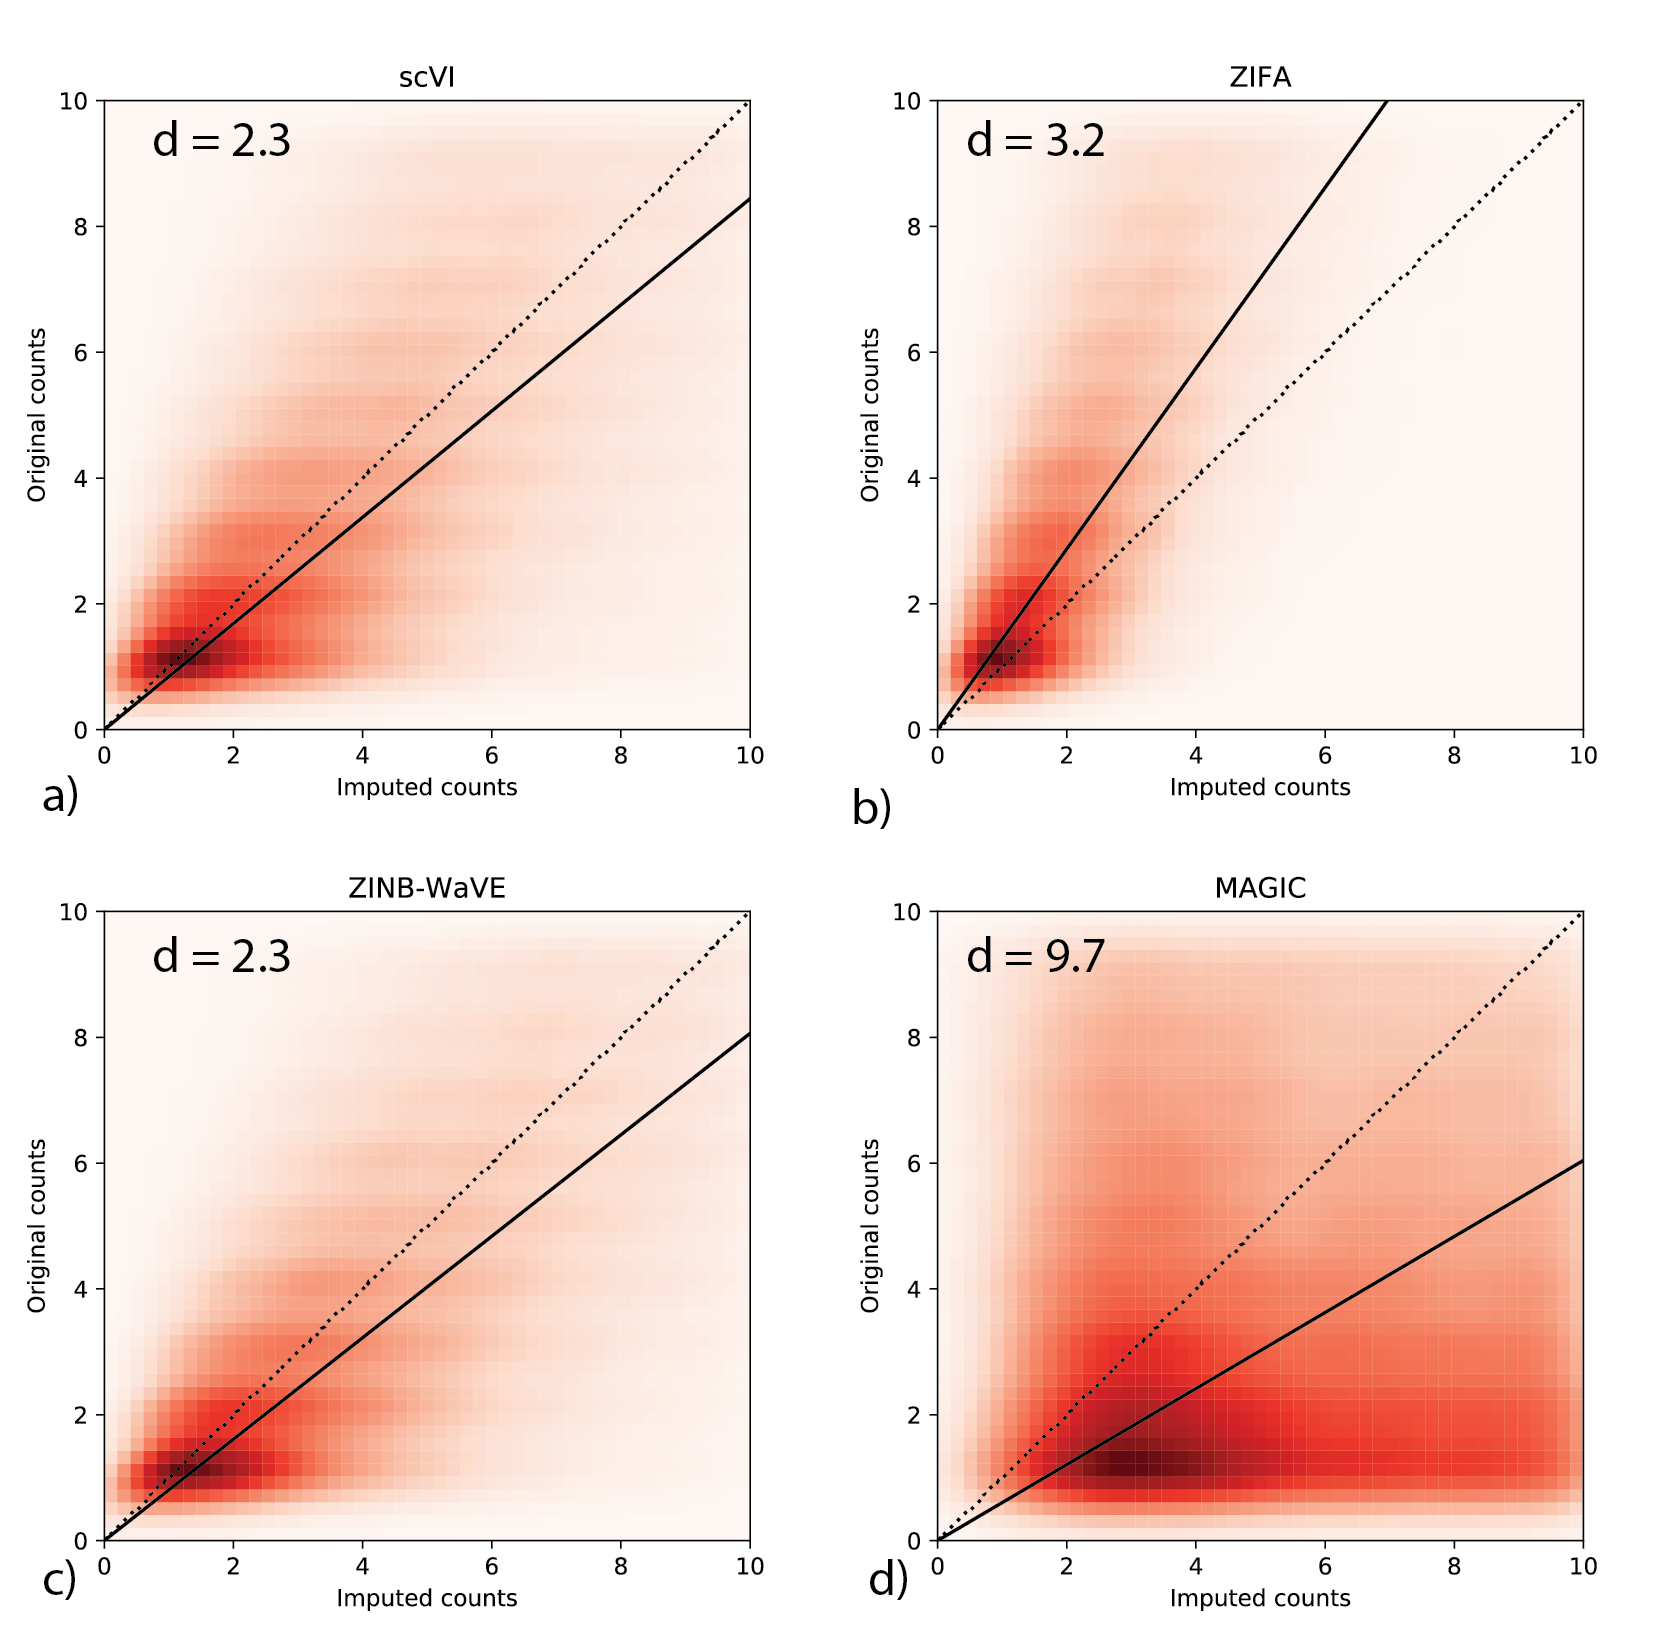
\includegraphics[width=\textwidth]{figures/Figure-3.png}
\caption[Imputation of scVI on the CORTEX dataset]{Imputation of scVI on the CORTEX dataset. The heatmaps denote density plots of imputed values (by scVI, ZIFA, MAGIC and ZINB-WaVE respectively) on a down-sampled version versus the original (non- zero) values prior to down-sampling. The reported score $d$ is the median imputation error across all the hidden entries (Lower is better; see Methods).}
\label{scviimpute_panel}
\end{figure}

To provide an example in which the perturbed values depend on the amount of mRNA observed, we also generated a corrupted training set by downsampling $10\%$ uniformly chosen non-zero entries with a binomial law of rate $20\%$. These values guarantee that most of the dataset is unchanged and require that the model has enough flexibility to impute correctly the changed values. With respect to these corruption scheme, scVI also performs well (Figure~\ref{scvilog_imputation_non_unif}, ~\ref{scvilog_imputation_non_unif_supp}).
% for revision, think about regularization on the dispersion parameters as in ZINB-WaVE
% Also, commenting on how imputation get worse with number of genes would help for understanding

scVI, like ZIFA and FA, can also be used to generate unseen data by sampling from the latent space. As evidence of the validity of this procedure, we sampled from the posterior distribution given the perturbed training data and observed that the samples are largely consistent with the unperturbed data (Figure~\ref{scviposterior_supp}).


\subsection{Capturing biological structure in a latent space}
\label{scviclustering_results}
To further assess the performance of scVI, we evaluated how well its latent space summarizes biological information and recovers biologically coherent subpopulations. For these experiments, we used three datasets where pre-annotated clusters or subpopulations are available: CORTEX, PBMC and RETINA. We then examined whether the annotated subpopulations were distinguishable in the latent space, as in \cite{Wang2017}. 

\subsubsection{Annotation-based evaluation metrics}
We report two different type of metrics for this analysis. The first is silhouette width~\cite{ROUSSEEUW198753}, which evaluates whether cells from the same subpopulation have a similar latent representation and cells from different subpopulations have a different representation. The silhouette width requires either a similarity matrix or a latent space. We can define a silhouette score for each sample $i$ with:
\begin{align}
    s(i) = \frac{b(i) - a(i)}{\max\{a(i),b(i)\}}, 
\end{align}
where $a(i)$ is the average distance of $i$ to all data points in the same cluster $c_i$ and $b(i)$ is the lowest average distance of $i$ to all data points in the same cluster $c$ among all clusters $c$. Clusters can be replaced with batches if we are estimating the silhouette width for assessing batch effects~\cite{SCONE}.

For the second metric, we used the latent representation as an input to the $K$-means algorithm (with $T=200$ random initializations to achieve a stable score), and measured the overlap between the resulting clustering annotations and the pre-specified subpopulations using the adjusted rand index (ARI) and normalized mutual information (NMI) scores. For ease of comparison across methods, we set $K$ to the number of annotated subpopulations.

The ARI is defined as:
\begin{align}
    ARI = \frac{\sum_{ij} \binom{n_{ij}}{2} - [\sum_i \binom{a_i}{2} \sum_j \binom{b_j}{2}] / \binom{n}{2} }{ \frac{1}{2} [\sum_i \binom{a_i}{2} + \sum_j \binom{b_j}{2}] - [\sum_i \binom{a_i}{2} \sum_j \binom{b_j}{2}] / \binom{n}{2}},
\end{align}
where $n_{ij}, a_i, b_j$ are values from the contingency table. 

The NMI is defined as 
\begin{align}
NMI = \frac{I(P;T)}{\sqrt{\mathbb{H}(P)\mathbb{H}(T)}}
\end{align}
where $P, T$ designates empirical categorical distributions for the predicted and real clustering. $I$ is the mutual entropy and $\mathbb{H}$ is the Shannon entropy.

\subsubsection{Annotation-agnostic evaluation metrics}
While these annotated subpopulations were subject to manual inspection and interpretation, a remaining caveat is that they are computationally derived. To address this, we make use of the CBMC dataset that includes measurements of thirteen key marker proteins in addition to mRNA. For evaluation, we quantify the extent to which the similarity between cells in the mRNA latent space resembles their similarity at the protein level. To this end, we compute the overlap fold enrichment between the protein and mRNA-based cell 100-nearest neighbor graph and the Spearman correlation of the adjacency matrices.
% For revision, consider running the p values (with tail of hypergeometric distribution)

\subsubsection{Results}

Based on these benchmarks, we compared scVI to other methods that aim to infer a biologically meaningful latent space (ZIFA, ZINB-WaVE, DCA, and FA), using the same clustering scheme. We find that scVI compares favorably to these methods for all of the datasets (Figure~\ref{scviclustering_supp}ab). Focusing on the PBMC dataset, we also compared scVI with a simpler version that does not explicitly model library size. Our results (Figure~\ref{scviclustering_supp}a) suggests that this additional modeling increases the clustering abilities of scVI. Next, we benchmark scVI with SIMLR \cite{Wang2017}, a method that couples clustering with learning a cell-cell similarity matrix. For the first set of tests, we set the number of clusters in SIMLR to be the true number of annotated subpopulations. For the CBMC case, we let SIMLR automatically determine that number. When we examine the evaluations that were based on the computationally derived annotations, we find that SIMLR outperforms scVI (Figure~\ref{scviclustering_supp}ab). However, while the latent space inferred by SIMLR provides a tight representation for these subpopulations, it may disregard other forms of critical information. Indeed, in the CBMC-based test, where the clustering is based on ``external'' but biologically meaningful data, scVI and DCA are the best performing methods, albeit by a small margin (Figure~\ref{scviclustering_supp}c).

\begin{figure}
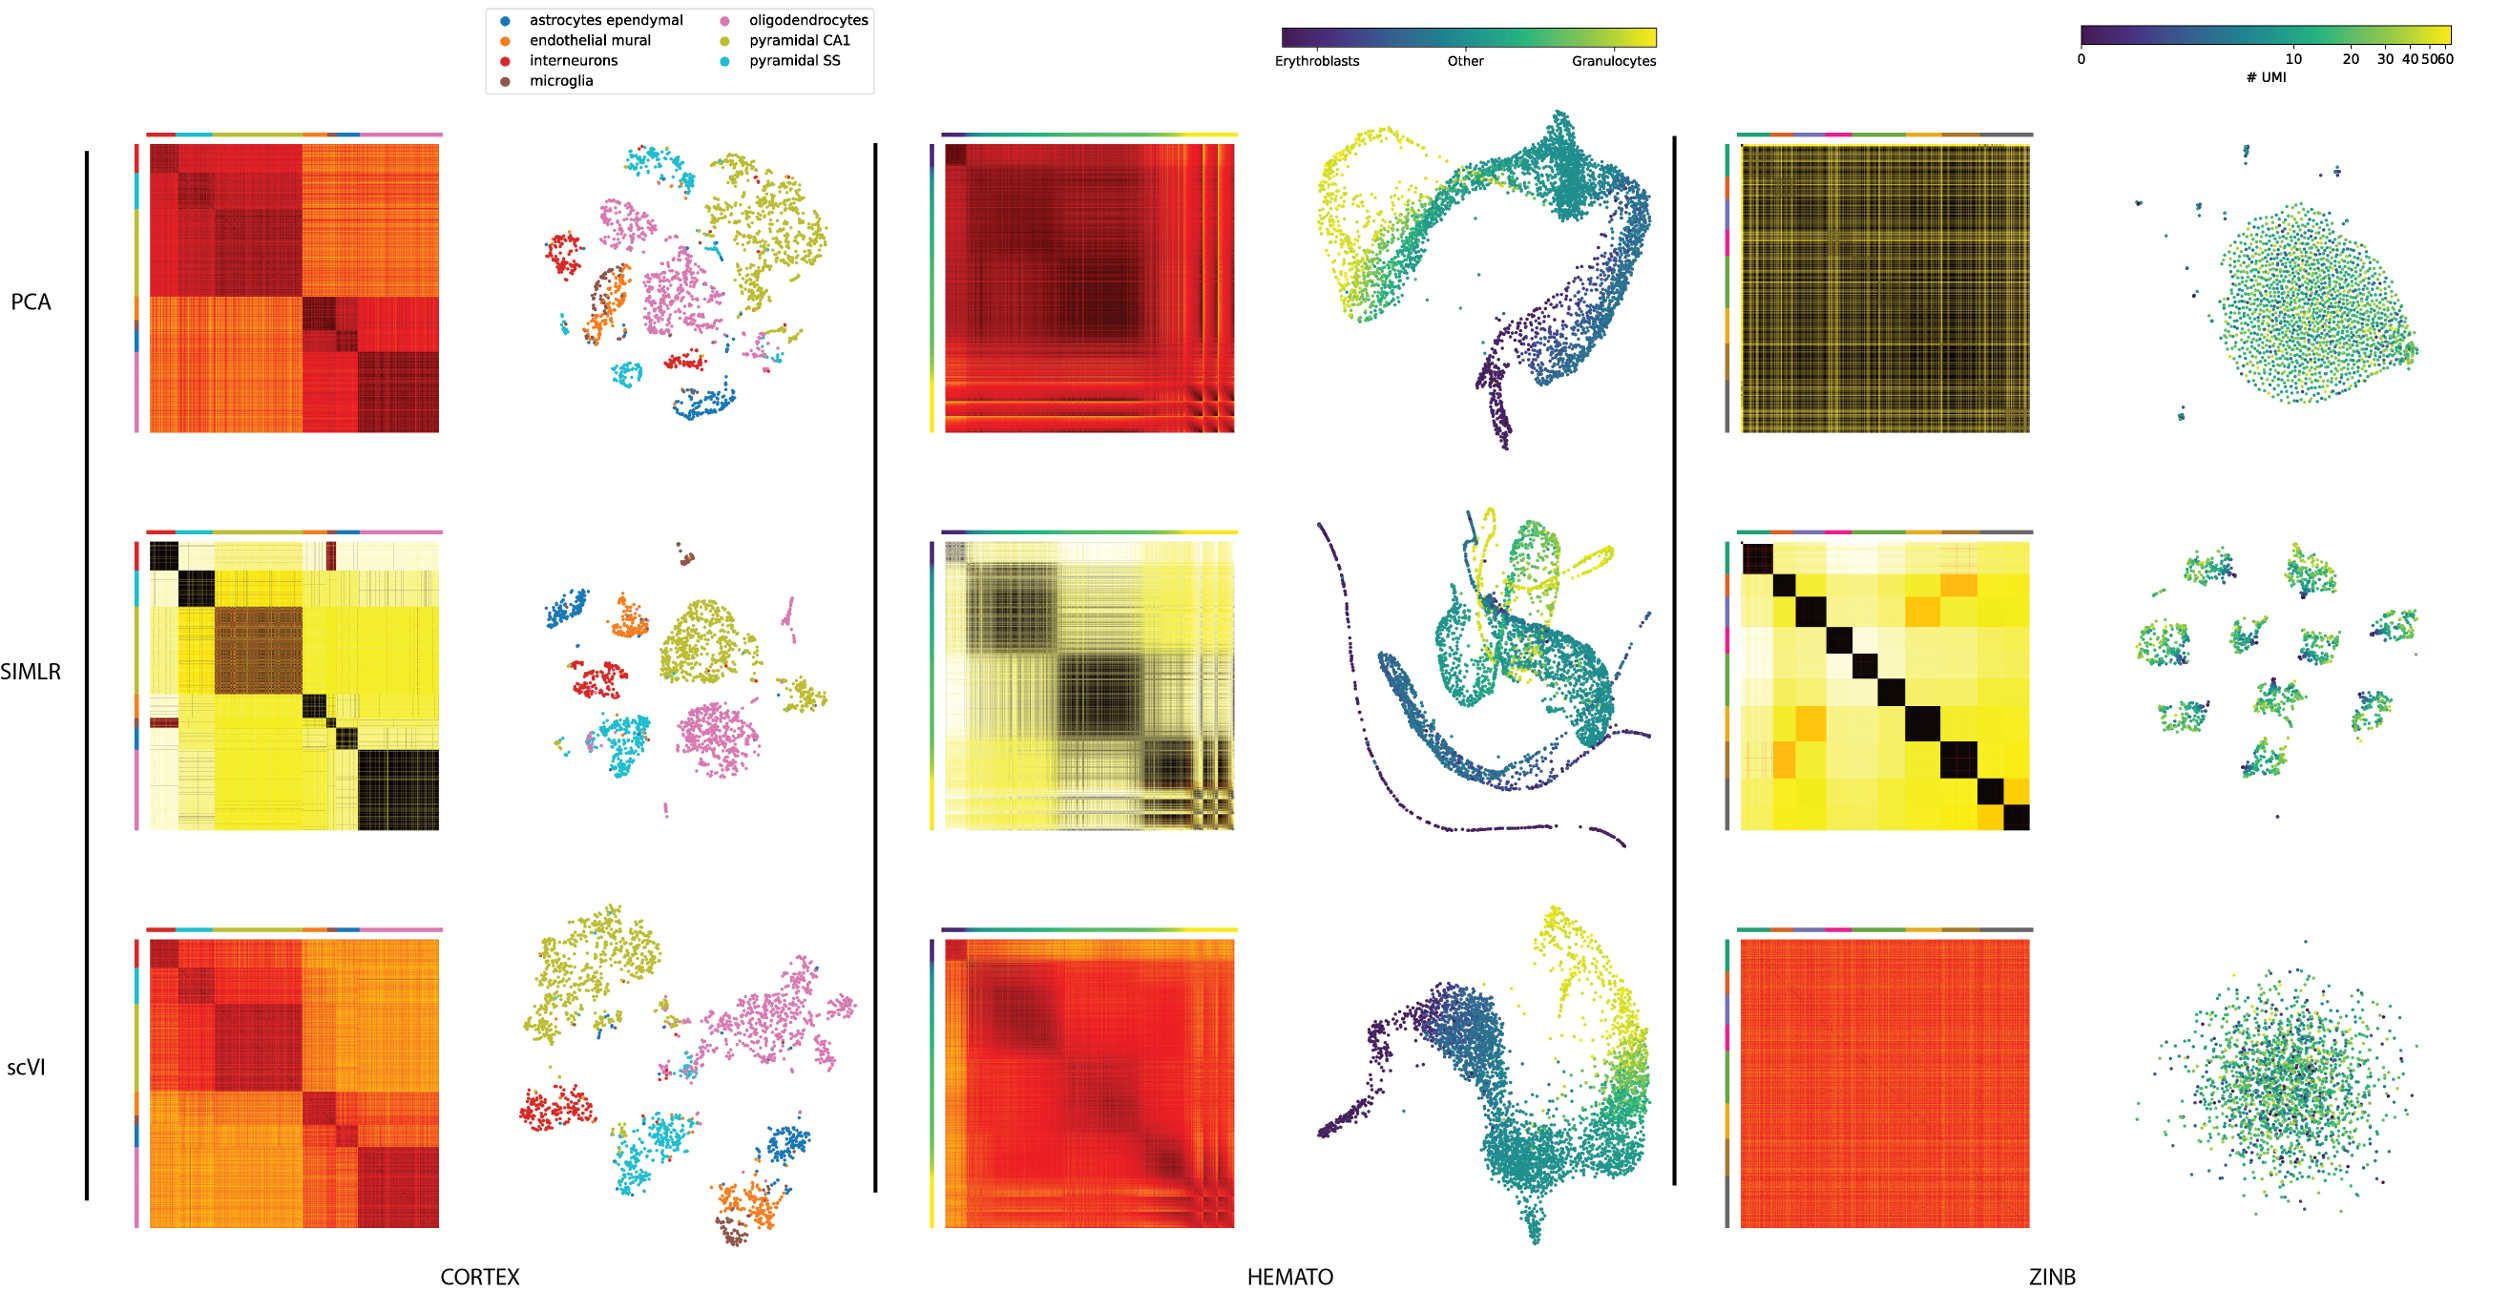
\includegraphics[width=\textwidth]{figures/Figure-2}
\centering
\caption[Clustering panel for scVI, PCA and SIMLR]{We apply scVI, PCA and SIMLR to three datasets (from right to left: CORTEX, HEMATO and a simulated `'noise'' dataset sampled iid from a fixed zero-inflated negative binomial (ZINB) distribution). For each dataset, we show a distance matrix in the latent space, as well as a two-dimensional embedding of the cells. Distance matrices: the scales are in relative units from low to high similarity (over the range of values in the entire matrix). For CORTEX and HEMATO, cells in the matrices are grouped by their pre-annotated labels, provided by the original studies (for the CORTEX dataset, cell subsets were ordered using hierarchical clustering as in the original study). For ZINB, the color in the distance matrices is determined by the clusters found by SIMLR on this data.  Embedding plots: each point represents a cell and the layout is determined either by tSNE (CORTEX, ZINB) or by a 5-nearest neighbors graph visualized using a Fruchterman-Reingold force-directed algorithm (HEMATO; see Figure~\ref{scvisuppfig2}d for the original embedding for SIMLR). For CORTEX and HEMATO, the color scheme in the embeddings is the same as in the distance matrices. For ZINB, the colors reflect the number of UMI in each cell (see Figure~\ref{scvisuppfig2}a-c for coloring of cells according to SIMLR clusters)}
\label{scviclustering_panel}
\end{figure}


Another example of important information that may be missed is the hierarchical structure among clusters, such as the one reported for the CORTEX dataset~\cite{Zeisel1138}. We take several cuts at different depths of the hierarchical clustering (Table~\ref{scvicortex-celltypes}) and report clustering scores based on these agglomerated labels (Figure~\ref{scviclustering_supp}efg). These results suggest that scVI and ZINB-WaVE find low-dimensional representations that better preserve this important biological structure.


A second important case occurs when the variation between cells has a continuous, rather than discrete, form. An example of this is the HEMATO dataset, which consists of hematopoietic cells annotated along seven different stages of differentiation. As a first step, we focus on cell development towards either granulocytic neutrophil or erythoid fate~\cite{Tusi2018}. SIMLR applied to this dataset predicts the presence of five clusters, and the resulting five-nearest-neighbors graph (visualized using a Fruchterman-Reingold force-directed algorithm) does not reflect the continuous nature of this system. Conversely, standard PCA analysis and scVI are able to capture this property of the data (Figure~\ref{scviclustering_panel}), albeit with less precision than the finely tuned process used in the original publication (Figure~\ref{scvihemato_supp}). 

Finally, there may be the case of lack of structure, where the data is almost entirely dominated by noise. To explore this setting, we generated a noise dataset, sampled at random from a vector of zero-inflated negative binomial distributions. SIMLR erroneously reports eleven distinct clusters in this data, which are not perceived by any other method (Figure~\ref{scviclustering_panel},~\ref{scvisuppfig2}a-c).

Altogether, these results suggest that the latent space of scVI is flexible and describes the data well, either as discrete clusters, as a continuum between cell state, or as structureless noise. scVI is therefore better suited than SIMLR in scenarios where the data does not necessarily fit with a simple structure of discrete subpopulations.


\subsection{Controlling for batch effects}
\label{scvibatch_results}
scVI explicitly accounts for the contribution of discrete nuisance factors of variation such as batch annotations in its graphical model. It does so by enforcing conditional independence between them and the inferred parameters.

\begin{figure}[htp]
\centering
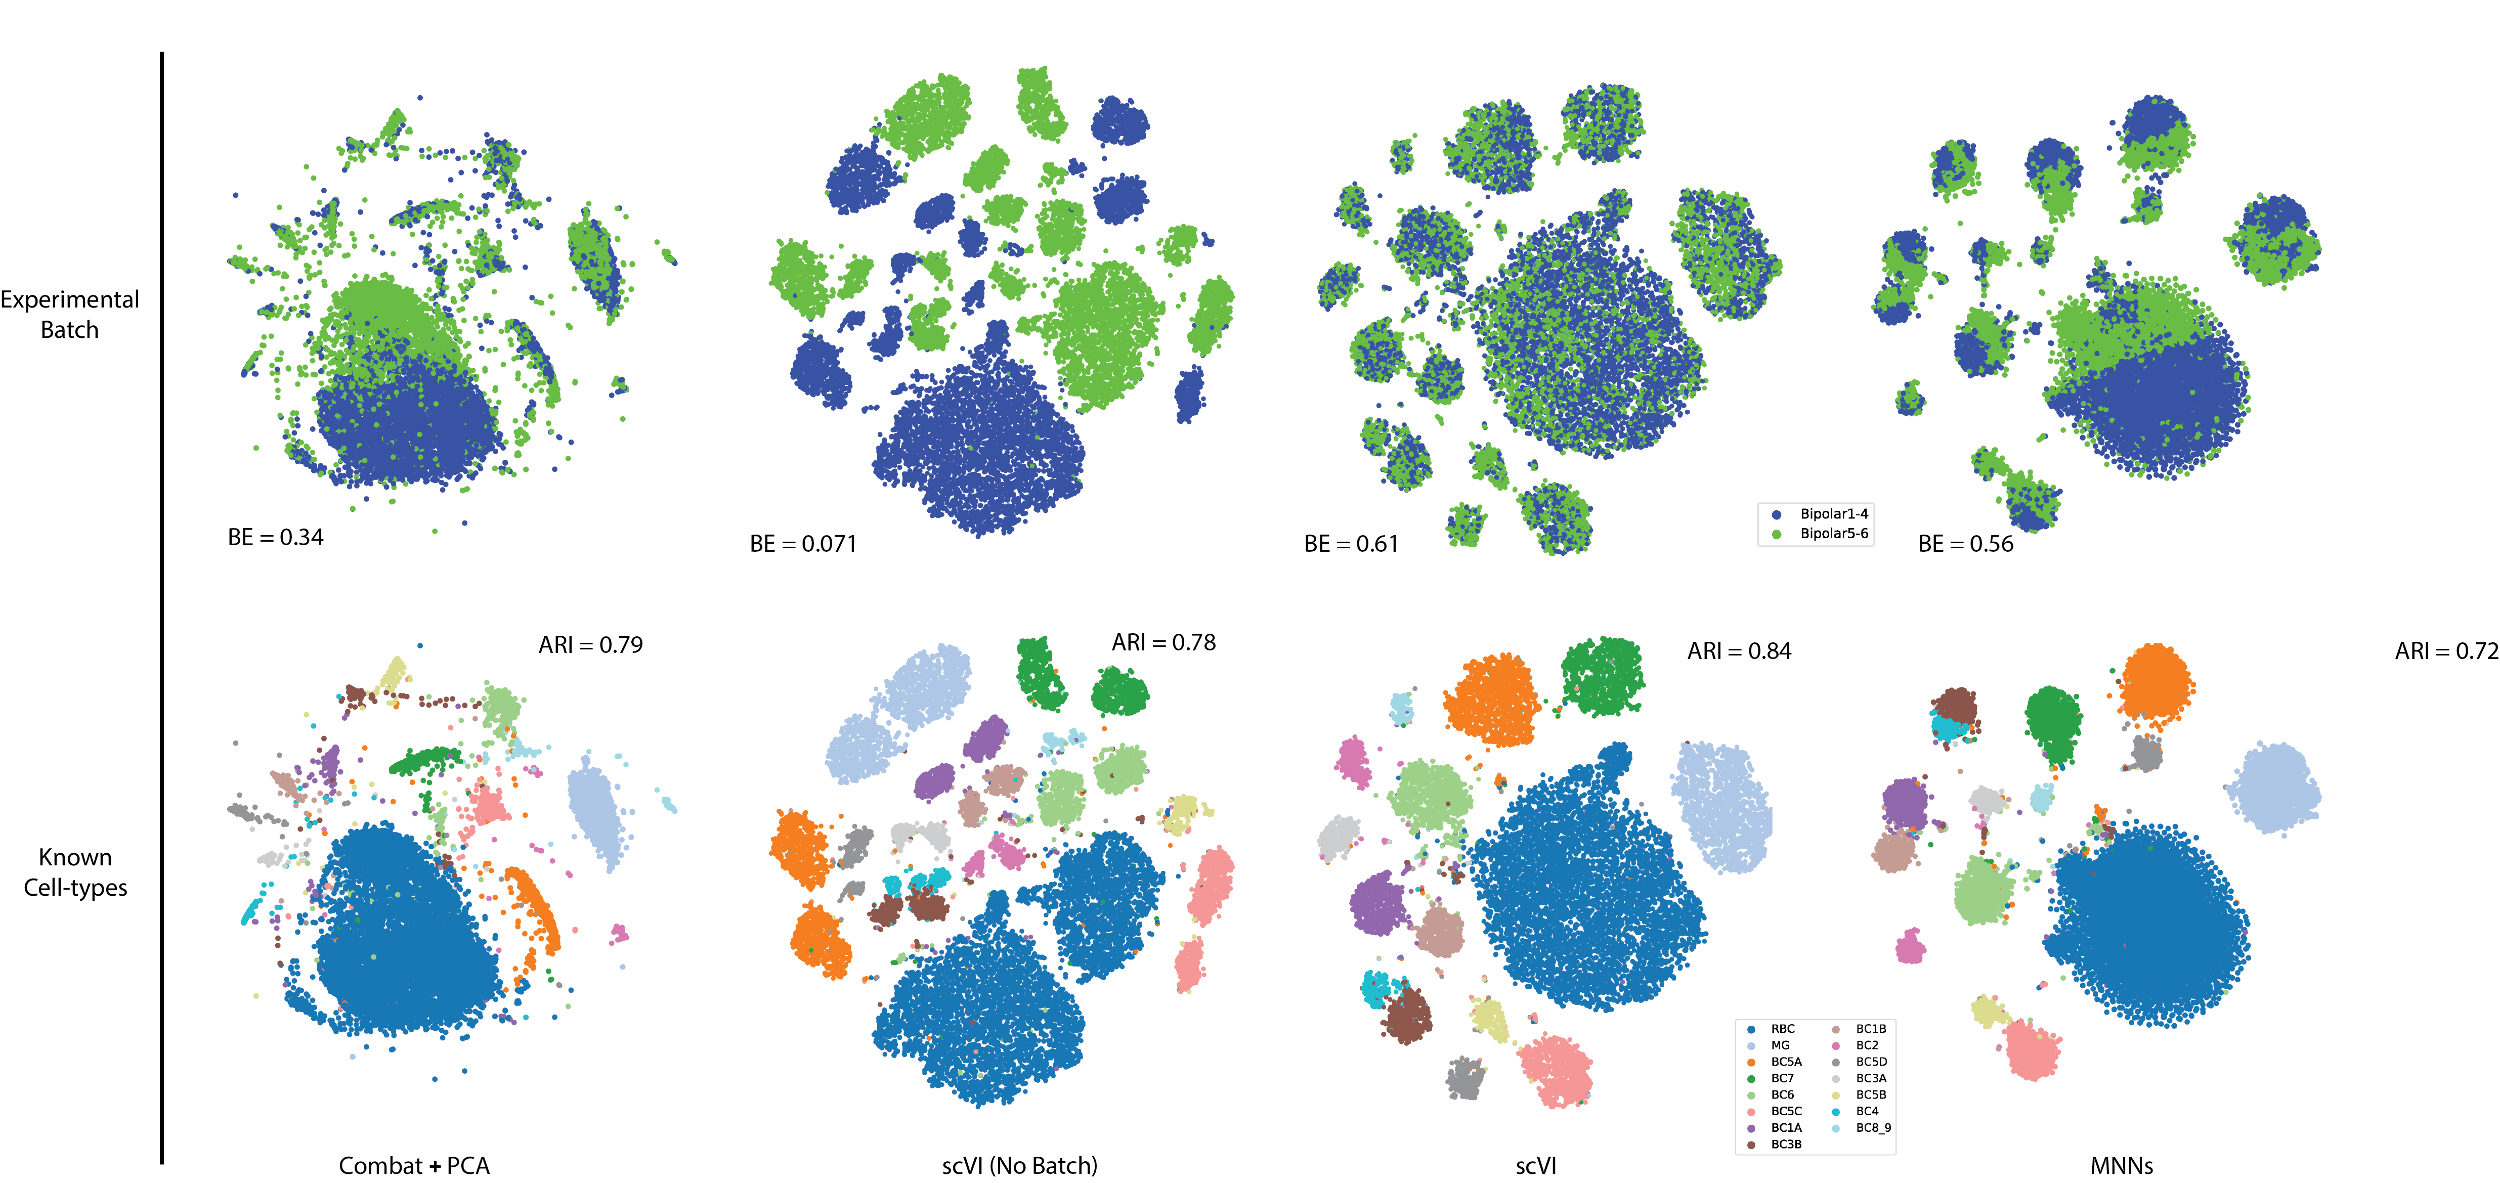
\includegraphics[width=\textwidth]{figures/Figure-5}
\caption[Batch effect removal with scVI on the RETINA dataset]{Batch effect removal with scVI on the RETINA dataset. We visualize the batch removal and clustering performance. A successful method renders a latent space which maintains a satisfactory level of clustering while sufficiently mixing the batches. Embedding plots (PCA with ComBat, scVI without batch correction, scVI and PCA with MNNs) were generated by applying tSNE on the respective latent space. In the upper part of the figure, the cells are colored by batch. In the lower part, cells are colored by the annotation of subpopulations, provided in the original study~\cite{bipolar}. For each algorithm, we report the batch entropy mixing for the batches (BE; higher is better) and the adjusted Rand index for the clustering (ARI; higher is better). When using PCA, we used the top 100 principal components (the top 10 resulted in no discernible structure).}
\label{scvibatch_panel}
\end{figure}

Our model therefore learns gene expression bias that comes from the batch effects and provides a parametric distribution that is disentangled from these technical effects, thus ideally reflecting the relevant biological variation. We evaluate the performance of scVI in correcting for batch effects using the RETINA dataset, which consists of two batches. We measured the entropy of batch mixing across the $K$-nearest neighbors graph with the ideal expectation of a uniform representation of batches (i.e., maximum entropy) in any local neighborhood. We also measure the average silhouette width; with no batch bias, batches should overlap perfectly and exhibit a null silhouette width. We compare our method to the more standard pipeline of batch correction ComBat~\cite{Johnson2007} followed by principal component analysis and the recent mutual nearest neighbors method (MNN~\cite{MNNpaper}). We also report results for methods that do not include batch correction in their underlying model, namely PCA, SIMLR, DCA and a simplified version of scVI with no conditioning for batches (Methods). Our results (Figure~\ref{scvibatch_panel},~\ref{scviclustering_supp}d,~\ref{scviMNNfigure}) demonstrate that in this dataset scVI aligns the batches better than Combat and MNN, while still maintaining a tight representation of pre-annotated subpopulations and compares favorably to all the other algorithms. Considering the latent space provided by algorithms without explicit batch modeling we find, as expected, that the mixing of the batches is poor. Specifically, while SIMLR and DCA are capable of clustering the cells well within each batch, the respective clusters from each batch remain largely separated. Furthermore, the poor batch mixing of the simplified scVI version demonstrates that the additional modeling complexity brought by the batch correction is important. Notably, we performed a similar analysis with the PBMC dataset, which consists of cells from two donors. However, this data seemed to exhibit only a minor batch effect to begin with (our metrics are averaged across all cell-types) and was thus less informative for the purpose of this evaluation  (Figure~\ref{scviclustering_supp}a).


\subsection{Differential expression}
\label{scvide_results}
Identifying genes that are differentially expressed between two subpopulations of cells is an important application of our generative model. The Bayesian model in scVI makes hypothesis testing straightforward. 

\subsubsection{A Bayesian hypothesis testing procedure for scVI}
For each gene $g$ and pair of cells ($z_a$, $z_b$) with observed gene expression $(x_a, x_b)$ and batch ID $(s_a, s_b)$, we can formulate two mutually exclusive hypotheses:
\begin{align}
    \mathcal{M}_1^g:= \mathbb{E}_sf_w^g(z_a, s) > \mathbb{E}_sf_w^g(z_b, s) \textrm{~~~~vs.~~~~} \mathcal{M}_2^g:=\mathbb{E}_sf_w^g(z_a, s) \leq \mathbb{E}_sf_w^g(z_b, s),
\end{align}
where the expectation $\mathbb{E}_s$ is taken with respect to the batch variable empirical frequencies. Notably, we propose a hypothesis testing that do not to calibrate the data to one batch but will find genes that are consistently differentially expressed. 
Again, evaluating the likelihood ratio test for whether our datapoints $(x_a, x_b)$ are more probable under the first hypothesis is equivalent to writing a Bayes factor~\cite{doi:10.1146/annurev-statistics-031017-100307}:
\begin{align}
K = \log_e \frac{p(\mathcal{M}_1^g \mid x_a, x_b)}{p(\mathcal{M}_2^g \mid x_a, x_b)}.
\end{align}
A Bayes factor is a Bayesian generalization of the p-value. Its sign indicates which of $\mathcal{H}_1^g$ and $\mathcal{H}_2^g$ is more likely. Its magnitude is a significance level and throughout the chapter, we consider a Bayes factor as strong evidence in favor of a hypothesis if $|K| > 3$~\cite{Kass1995} (equivalent to an odds ratio of $exp(3)\approx 20$).

The posterior of these models can be approximated by integrating against the variational distribution:
\begin{align}
p(\mathcal{M}_1^g \mid x_a, x_b) \approx \sum_s\iint_{z_a, z_b} p(f_w^g(z_x, s) \leq f_w^g(z_x, s) )p(s)dq(z_a \mid x_a)dq(z_b \mid x_b).
\end{align}
Here $p(s)$ designates the relative abundance of cells in batch $s$ and all of the measures are low-dimensional, so we can use naive Monte Carlo to compute these integrals. We can then use a Bayes factor for the test.

Since we assume that the cells are i.i.d., we can average the Bayes factors across a large set of randomly sampled cell pairs, one from each subpopulation. The average factor will provide an estimate of whether cells from one subpopulation tend to express $g$ at a higher frequency. 


\subsubsection{Benchmarking on real data}
We demonstrate the robustness of our method by repeating the entire evaluation process and comparing the results (Figure~\ref{scvibayes_panel}ab). We also ensure that our Bayes factor are well calibrated by running the differential expression analysis across cells from the same cluster and making sure no genes reach the significance threshold (Figure~\ref{scvibayes_supp}e).

To evaluate scVI as a tool for differential expression, we used the PBMC dataset along with its classification of cells into well-studied subtypes of hematopoietic cells, for which reference bulk expression data is available. 

\begin{figure}
    \centering
    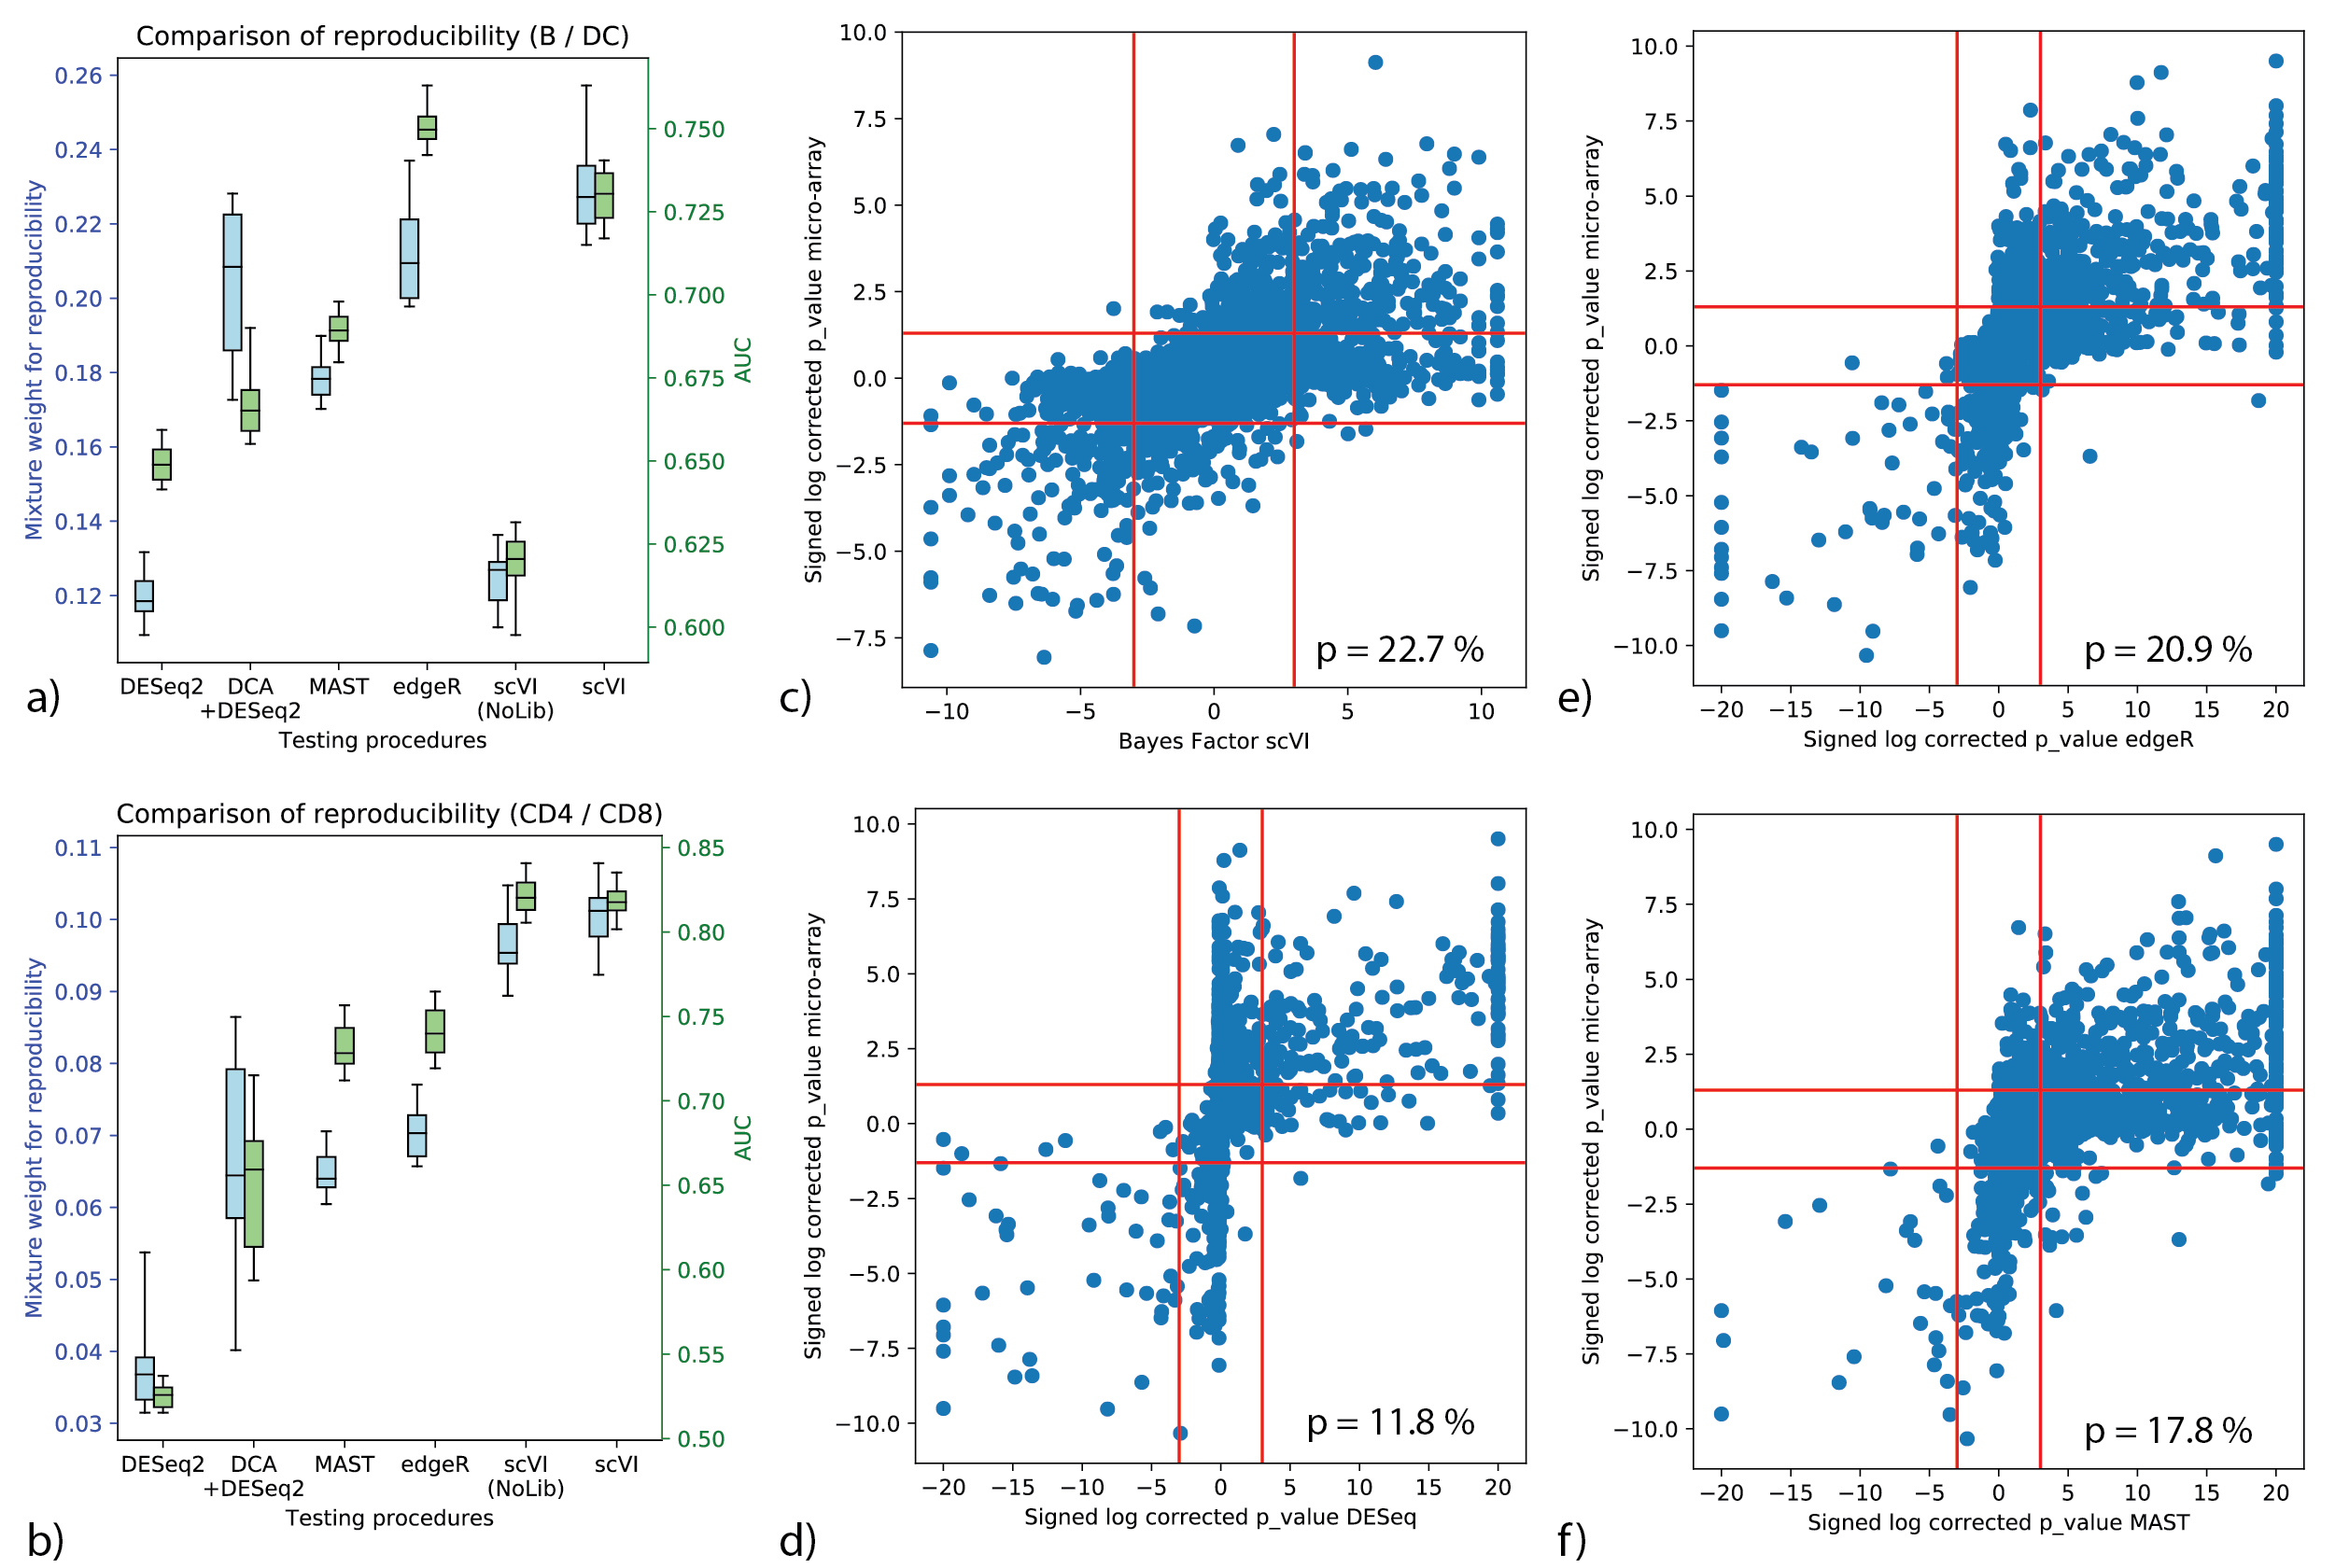
\includegraphics[width=\textwidth]{figures/Figure-4.png}
    \caption[Benchmark of differential expression analysis using the PBMC dataset]{Benchmark of differential expression analysis using the PBMC dataset, based on consistency with published bulk data. (a, b) Evaluation of consistency with the irreproducible discovery rate (IDR)~\cite{Li2011} framework (blue) and using AUROC (green) is shown for comparisons of B cells vs Dendritic cells (a) and CD4 vs CD8 T cells (b). Error bars are obtained by repeatedly sub-sampling the data to show robustness. Whiskers denote the 5th and 95th percentiles.  (c,d,e,f): correlation of significance levels of differential expression of B cells vs Dendritic cells, comparing bulk data and single cell. Points are individual genes. Bayes factors or p-values on scRNA-seq data are presented on the x-axis; microarray-based  p-values are depicted on the y-axis. Horizontal bars denote significance threshold of 0.05 for corrected p-values. Vertical bars denote significance threshold for the Bayes factor of scVI (c) or 0.05 for corrected p-values for DESeq2 (d), edgeR (e), and MAST (f). We also report the median mixture weight for reproducibility $p$ (higher is better).}
    \label{scvibayes_panel}
    \end{figure}

We compare scVI to three widely used methods: DESeq2~\cite{deseq2}, MAST~\cite{mast} and edgeR~\cite{edgeR}. We also compare scVI to a simpler version of the model in which we do not explicitly model library size. Finally, we compare to a hybrid method where the counts are first imputed by DCA and then used for differential expression with DESeq2, as proposed by the authors~\cite{dca}. To facilitate the evaluation, we defined a reference set of differentially expressed genes using publicly available bulk expression datasets. Specifically, we assembled a set of genes that are differentially expressed between human B cells and dendritic cells (microarrays, n=10 in each group~\cite{Nakaya2011}) and between CD4+ and CD8+ T cells (microarrays, n=12 in each group~\cite{Gorgun2005}). We apply all six methods in these two differential expression tasks (using the respective clusters of cells) and evaluate the consistency with the reference data using two scores. For the first score, we assign each gene with a label of DE or non-DE based on their p-values from the reference data (genes with a corrected p-values under $0.05$ are positive and the rest are negative); then these labels to compute AUROC for scVI and each of the benchmark methods.
% we could use the genes from GSE to have a better negative set, or think about a signed p value ranking

Since defining the labels requires a somewhat arbitrary threshold,  we use a second score that evaluates the reproducibility of gene ranking (bulk reference vs. single cell; considering all genes), using the irreproducible discovery rate (IDR)~\cite{Li2011}. Considering the AUROC metric, scVI is the best performing method in the T cell comparison, while edgeR outperforms scVI by a smaller margin in the B vs. dendritic cell comparison. Considering the proportion of genes with reproducible rank as fitted by IDR, scVI is the best performing method in both comparisons (Figure~\ref{scvibayes_panel}, Figure~\ref{scvibayes_supp}a-d). Interestingly, the simpler scVI model shows extremely poor performance on the B vs. dendritic cell comparison, being the only model that does not explicitly handle normalization. This is evidence of the usefulness of explicitly including library size normalization in the scVI model. Furthermore, we see that the hybrid method of DCA followed by DESeq2 constitutes a solid improvement over a direct application of DESeq2; however, the performance is still lower than other methods. 
%Taken together, these results suggest that combining models without compatible statistical assumptions might result in a loss of statistical power, hence the advantage of performing all the relevant tasks under the same Hierarchical Bayes model. %NIR: I am not sure what you are referring to here. Is this really an issue with the benchmark methods? %ROMAIN: Let us dump that.


\subsection{Capturing technical variability}
\label{scvitechnicalnoise_results}
To further interpret the fitted models, we study the extent to which they capture technical variability. We focus on datasets that were generated by 10x, as they share the same set of cell quality metrics (generated by cell ranger) and can thus provide reproducible insights about the relationship between our parameters and library quality. Additionally, we required our test datasets to have pre-annotated subpopulations, with the assumption that each subpopulation consists primarily of cells of the same type, thus decreasing the extent of biological heterogeneity (e.g., in total mRNA content). The two datasets that fit these requirements, which we report next, are the PBMC and BRAIN-SMALL.

In each case, we trained the model on the entire dataset and then investigated each pre-annotated subpopulation separately. As a general rule, we find that variation in library size correlates strongly with the cell-specific scaling factor, which is to be expected by the definition of the model. Figure~\ref{scvinoise-model}a depicts these results for the CD14+ monocytes subpopulation in the PBMC data (notably, the negative curvature on the plot can be explained by shrinking the values towards the mean due to the use of a prior). Another important nuisance factor to be considered is the limitation in sensitivity, which exacerbates the number of zero entries. In principle, zero entries can be captured by two different components of our model: the negative binomial and the \enquote{inflation} of zeros added to it with a Bernoulli distribution. Evidently, the expected number of zeros generated by the negative binomial for each cell correlates strongly with the library size and its proxies (e.g., the number of detected genes or the number of reads per UMI; Figure~\ref{scvinoise-model}cd,~\ref{scviparameters_supp}d). This result can be explained by our definition of the negative binomial mean, which is the predicted frequency of expression $\rho_n^g$ scaled by the respective library size $\ell_n$.

The remaining question is therefore, what is the relationship between the expected frequency of expression $\rho_n^g$ and the observed zeros? A simple model would consist of a random process of sampling genes from each cell, in a manner proportional to their frequency, and with no added bias (e.g., in capture efficiency). To explore this, for every gene we plot the mean expected frequency against the percent of detecting cells in a subpopulation of interest (Figure~\ref{scvinoise-model}b). The resulting trend supports this simple model as it closely fits with the zero probability of a hypergeometric distribution---namely, random sampling of molecules without replacement.

Interestingly, the number of additional zeros induced by the Bernoulli random variable in each cell is less correlated with library size, and instead correlates with metrics of alignment rate (Figure~\ref{scvinoise-model}cd,~\ref{scviparameters_supp}cd). These metrics are not necessarily coupled to size, but may reflect other technical factors such as contamination or the presence of degraded mRNA. However, we observed that most zero values in the data can be explained by the negative binomial component alone (Figure~\ref{scviparameters_supp}a). Taken together, these results therefore corroborate the idea that most zeros, at least in the datasets explored here, can be explained by low (or zero) ``biological'' abundance of the respective transcript, which is exacerbated by limited sampling. 


\begin{figure}
\centering
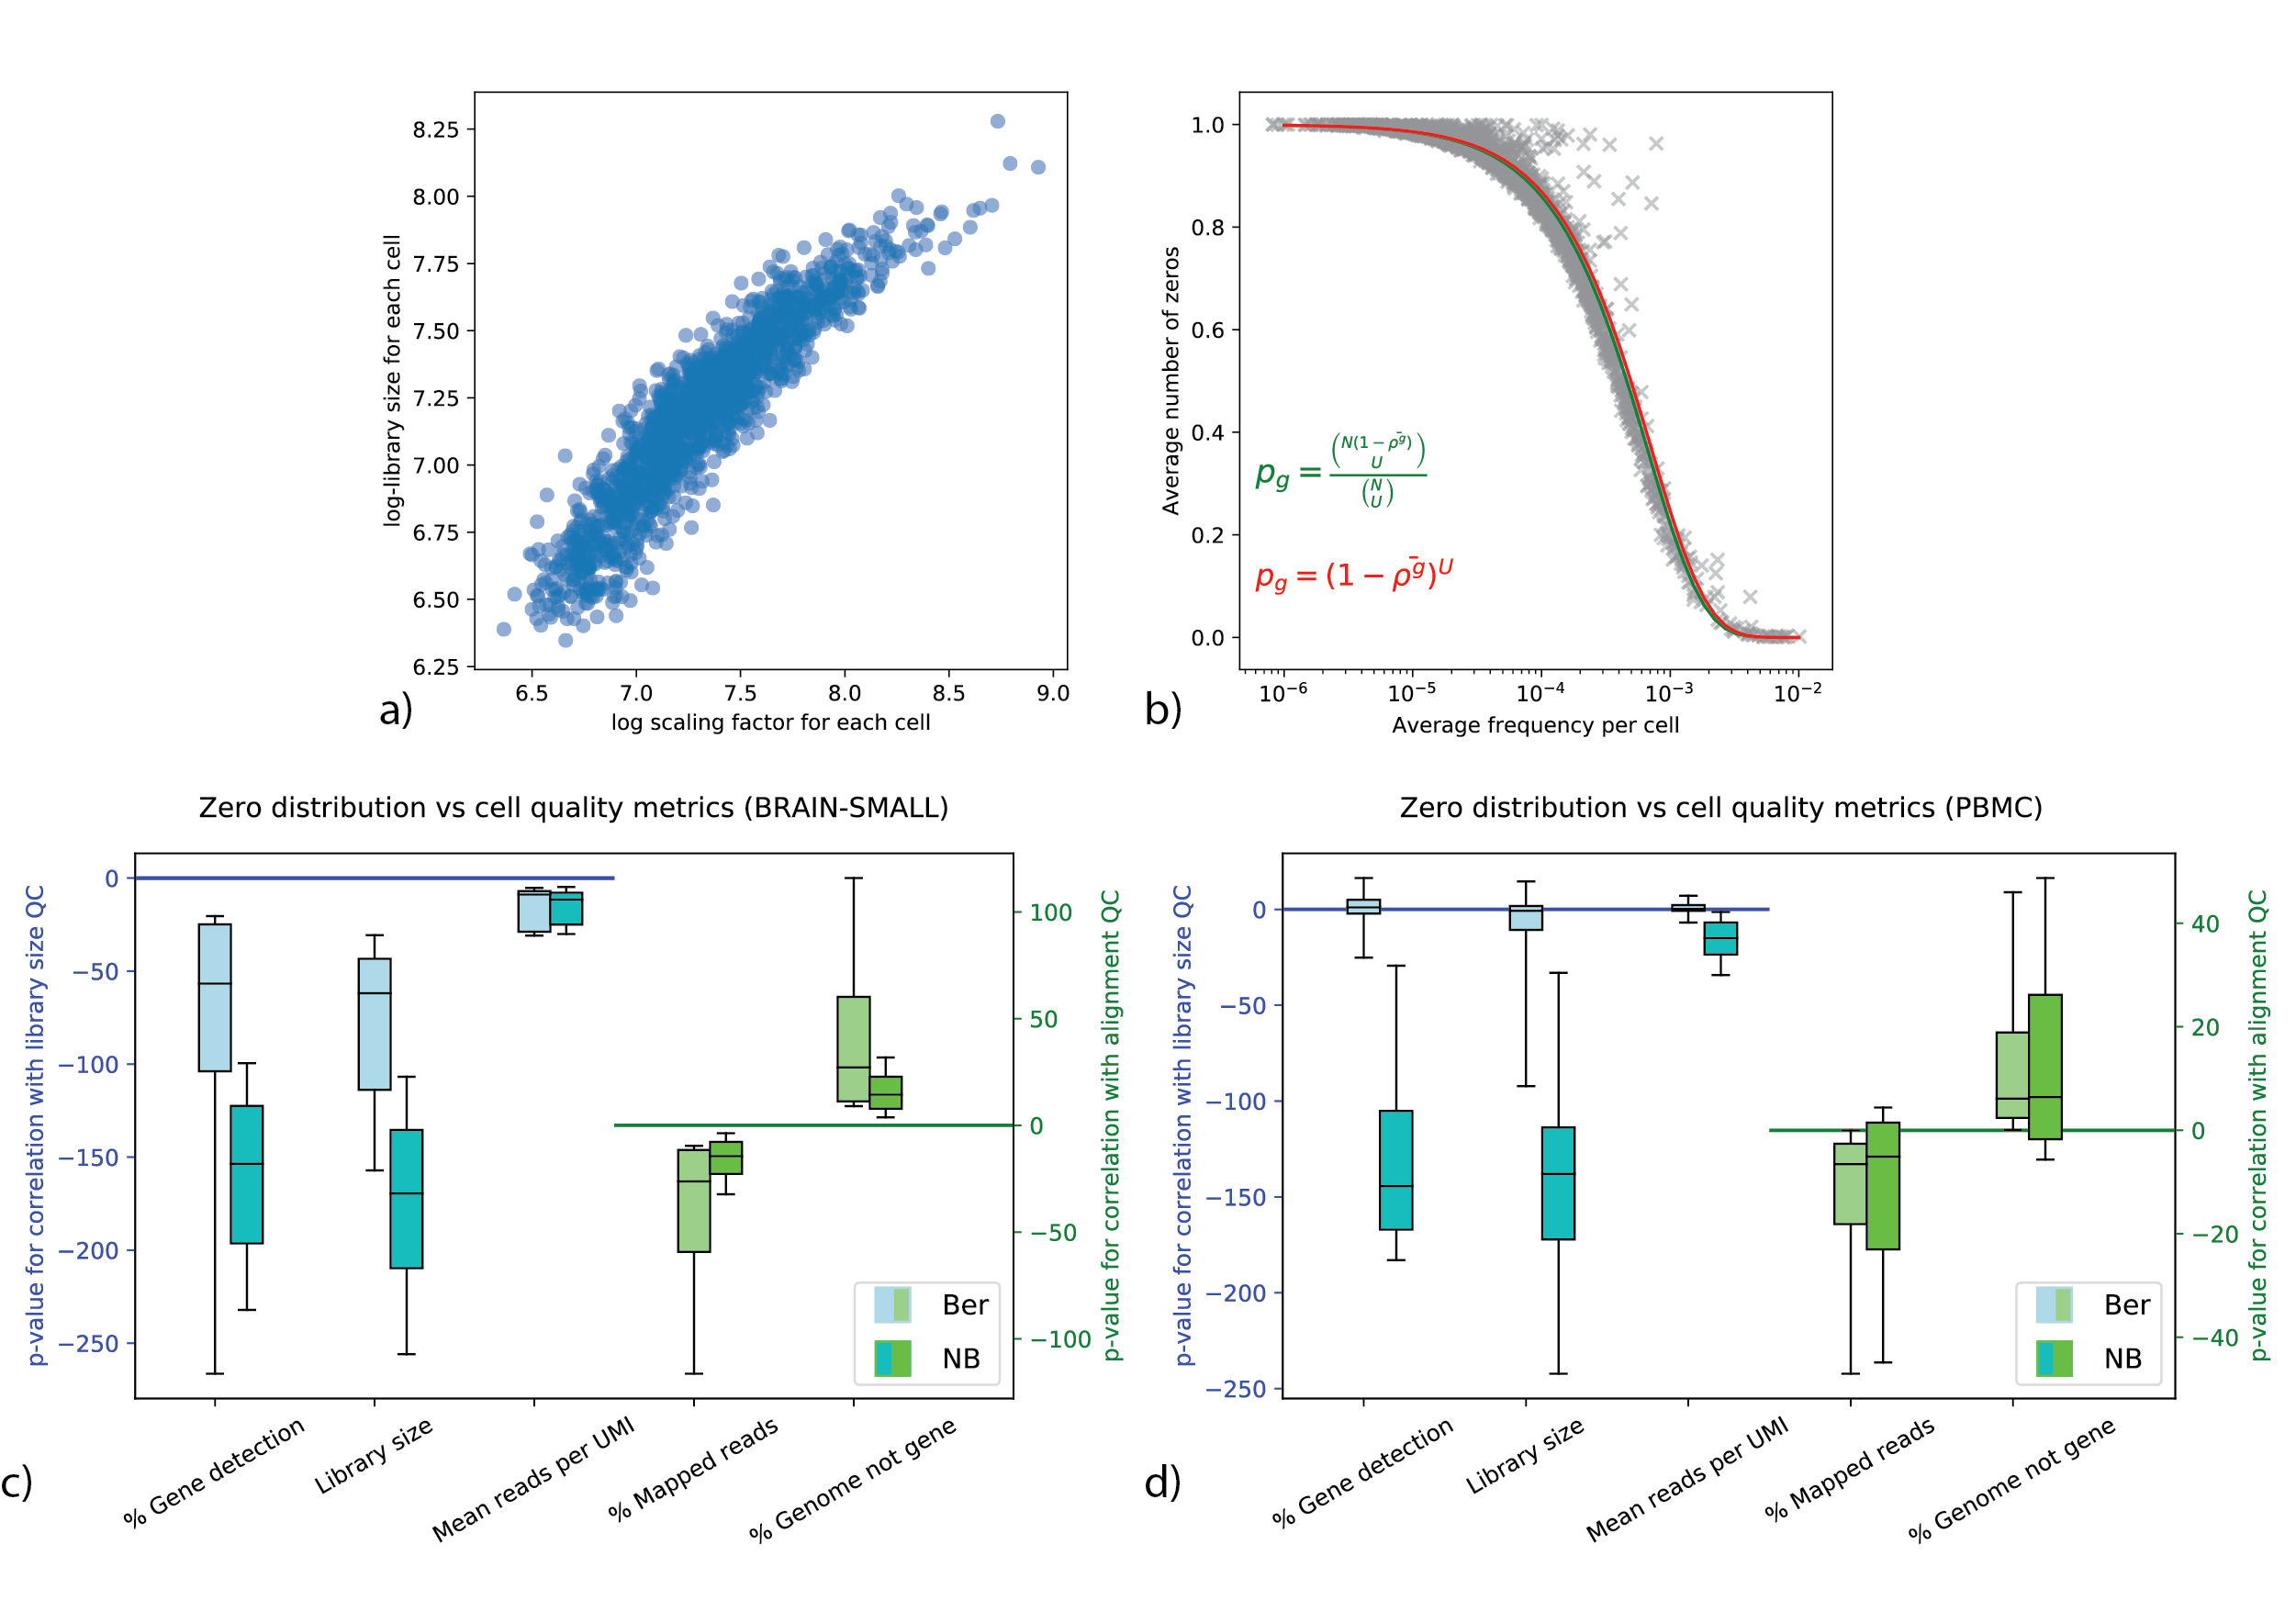
\includegraphics[width=0.95\textwidth]{figures/Figure-6.png}
\caption[Capturing technical variability using scVI]{Capturing technical variability using scVI. Data for panels a-b is based on the CD14+ cell subpopulation of the PBMC dataset. (a) Scatter plot for each cell of inferred scaling factor using scVI against library size. 
% Change the axis
(b) The frequency of observed zero values versus the expected expression level, as produced by scVI. Each point represents a gene $g$, where the x-axis is $\bar{\rho^g}$---the average expected frequency per cell (for gene $g$, average over $\rho_c^g$ for all cells $c$ in the subpopulation), and the y-axis the is observed percentage of cells that detect the fee (UMI>0). The green curve depicts the probability for selecting zero transcripts from every gene as a function of its frequency, assuming a simple model of sampling $U$ molecules from a cell with $N$ molecules at random without replacement. $U=1398$ is the average number of UMIs in the subpopulation and $N$ is the average number of transcripts per cell (for this curve $N=10k$). Notably, the curve converges for values larger than $20k$ to the red curve, a binomial selection procedure (conform to the probabilistic limit of the sampling process when $N\rightarrow \infty$). (c, d) Signed log p-values for testing correlations between the zero probabilities from the two distributions (negative binomial, Bernoulli) and quality control metrics across five random initializations of scVI and all subpopulations of the PBMC and BRAIN-SMALL datasets. Whiskers denote the 5th and 95th percentiles.}
\label{scvinoise-model}
\end{figure}


\subsection{Alternative modeling choices}
We consider here the extent to which each of a sequence of modeling choices in the design of scVI contributes to its performance. As a baseline approach, consider normalizing single-cell RNA sequencing data as in previous literature~\cite{zifa} and reducing the dimensionality of the data using a variational autoencoder with a Gaussian prior and a Gaussian conditional probability. 
    
One way in which a model can be enhanced is by changing the Gaussian conditional probability to one of the many available count distributions, such as zero-inflated negative binomial (ZINB), negative binomial (NB), Poisson or others. Recent work by Eraslan and colleagues using simulated data shows that when the dropout effect drives the signal-to-noise ratio to a less favorable regime, a denoising autoencoder with mean squared error (i.e., Gaussian conditional likelihood) cannot recover cell-types from expression data while an autoencoder with ZINB conditional likelihood can~\cite{dca}. This results points to the importance of at least modeling the sparsity of the data and is consistent with previous contributions~\cite{zifa,zinbwave}. 
    
The next question is which count distribution to use. In scVI we have chosen to use the zero-inflated negative binomial, a choice motivated by previous literature (e.g.,~\cite{zinbwave}). First, the choice of negative binomial is common in RNA-sequencing data, as it is over dispersed~\cite{deseq2}. Furthermore, under some assumption this distribution captures the steady state form of the canonical two-state promoter activation model~\cite{Grun2014}. Finally, recent work by Gr{\o}nbech and colleagues~\cite{scVAE} proposes an analysis based on Bayesian model selection (held-out log-likelihood as in this manuscript). In that analysis, the NB and ZINB distribution stand out with similarly high scores. We demonstrate that the addition of a zero-inflation (Bernoulli) component is important for explaining a subset of the zero values in the data (Figure~\ref{scviparameters_supp}) and that it captures important aspects of technical variability which are not captured by the NB component (Figure~\ref{scvinoise-model}).
    
To enhance the model further, we added terms to account for library-size as a nuisance factor, which can be considered as a Bayesian approach to normalization as in~\cite{biscuit,basics}. We showed how this contributes to our model by increasing clustering scores and the accuracy of differential expression analysis.
    
As a further enhancement, we designed the generative model to explain data from different experimental batches. This is not a trivial task as there may exist a significant covariate shift between the observed transcript measurements. We also showed how this modification to our model is crucial when dealing with batch effects.